\section{Introduction}

\subsection{Motivation}

There is increasing interest in the use of simulation-based models for obtaining \emph{causal} insights.
Such models aim to describe what \emph{would} occur when different actions or interventions are applied to some real-world process of interest, thereby allowing planning and decision-making to be done with a fuller understanding of the different outcomes that may result.
% to some real-world process of interest, and not simply the behaviour of the process as it evolves in isolation.
In many applications, models of this kind are referred to as \emph{digital twins} \citep{barricelli2019survey,jones2020characterising,niederer2021scaling}.
% A \emph{digital twin} is a virtual system that runs alongside some physical process of interest and mimics its behaviour over time in response to user-provided interventions. 
These have been considered for a wide range of use-cases including aviation \citep{tuegel2011reengineering}, manufacturing \citep{lu2020digital}, healthcare \citep{corral2020digital,coorey2022health}, civil engineering \citep{sacks2020construction}, and agriculture \citep{jans2020digital}.
% For a comprehensive overview, we refer the reader to 
% \emph{Digital twins} provide the ability to interact in real-time with a virtual clone of some real-world process of interest.
% This modelling approach promises to transform planning and decision-making across a breadth of fields, since it allows actions to be chosen with a fuller understanding of the range of possible outcomes that may result. % given the currently available data.

Many applications of digital twins are considered safety-critical, which means the cost of deploying an inaccurate twin to production is potentially very high.
% As such, methodology for assessing the performance of a twin before its deployment is essential for the safe adoption of digital twins in practice, and to ensure their far-reaching potential benefits can be fully realised.
As such, methodology for assessing the performance of a twin before its deployment is essential for the safe, widespread adoption of digital twins in practice \citep{niederer2021scaling}.
In this work, we consider the problem of assessing twin accuracy and propose a concrete, theoretically grounded, and general-purpose methodology to this end.
We focus specifically on the use of statistical methods that leverage data obtained from the real-world process that the twin is designed to model.
Such strategies are increasingly viable for many applications as datasets grow larger, and offer the promise of lower overheads compared with alternative strategies that rely for instance on domain expertise.

We formulate twin assessment as a problem of \emph{causal inference} \citep{rubin1974estimating,rubin2005causal,pearl2009causality,hernan2020causal}.
In particular, we consider a twin to be accurate if it correctly captures the behaviour of a real-world process of interest in response to certain interventions, rather than the behaviour of the process as it evolves on its own.
This seems in keeping with the overall (if often implicit) design objectives that underlie many applications, including those cited above.
% As well as providing a precise framework within which to consider twin assessment, an explicitly causal approach also highlights certain pitfalls that arise when conventional, non-causal approaches are applied to this problem.
% As well as supplying a precise framework for twin assessment,
Our causal assessment approach also highlights certain pitfalls associated with conventional methods that do not account for causal factors, and that can give rise to misleading inferences about the twin as a result.

% We adopt the position that in order to be considered ``accurate'', a twin must correctly capture the causal effects of interventions applied to the real-world process of interest. Naturally, this means that twin assessment can be formulated as a problem of \emph{causal inference} \citep{rubin1974estimating,rubin2005causal,pearl2009causality,hernan2020causal}, which offers a particularly suitable framework for reasoning about interventional behaviour of this kind.

% A principal design objective for digital twins is to improve decision-making, with much emphasis placed on their ability to reveal choices of actions that are expected to produce some desirable outcome in the real world \citep{barricelli2019survey,jones2020characterising,niederer2021scaling}.

% Since digital twins are designed to improve decision-making, in order to be considered ``accurate'', they must capture the range of outcomes that \emph{would} occur when certain actions or interventions are applied to the real-world process of interest in a controlled way. %, rather than the outcomes that \emph{are observed} to occur as the process evolves on its own.
% % Accordingly, we formulate twin assessment within the framework of \emph{causal inference} \cite{rubin1974estimating,rubin2005causal,pearl2009causality,hernan2020causal}, which provides a precise mathematical language for posing interventional or ``What if?''-type questions about a system, and for answering these questions to the extent possible via statistical methods applied to real-world data.
% Accordingly, we formulate twin assessment as a problem of \emph{causal inference} \citep{rubin1974estimating,rubin2005causal,pearl2009causality,hernan2020causal}, which offers a particularly suitable framework for reasoning about interventional behaviour of this kind.


% \rob{Rather than describing the behaviour of some real-world process as it evolves in isolation,}
% A principal design objective for digital twins is to improve decision-making, with much emphasis placed on their ability to reveal choices of actions that are expected to produce some desirable outcome in the real world \citep{barricelli2019survey,jones2020characterising,niederer2021scaling}.
% We therefore adopt the position that, to be considered ``accurate'', a twin must capture the range of outcomes that \emph{would} occur when certain actions or interventions are applied to the real-world process of interest in a controlled way. %, rather than the outcomes that \emph{are observed} to occur as the process evolves on its own.
% % Accordingly, we formulate twin assessment within the framework of \emph{causal inference} \cite{rubin1974estimating,rubin2005causal,pearl2009causality,hernan2020causal}, which provides a precise mathematical language for posing interventional or ``What if?''-type questions about a system, and for answering these questions to the extent possible via statistical methods applied to real-world data.
% Accordingly, we formulate twin assessment as a problem of \emph{causal inference} \citep{rubin1974estimating,rubin2005causal,pearl2009causality,hernan2020causal}, which offers a particularly suitable framework for reasoning about interventional behaviour of this kind.

% The primary reason for assessing the accuracy of a twin is to determine its reliability and robustness.
In most cases, it is desirable for an assessment procedure to be reliable and robust, and for its conclusions about the twin to be highly trustworthy.
% As such, it is intuitively desirable for any information obtained via our assessment procedure to be highly trustworthy.
% As such, we aim to obtain an assessment procedure that requires minimal assumptions about the twin and the real-world process it is designed to model.
As such, our goal in this paper is to obtain a methodology that is always \emph{sound}, even possibly at the expense of being conservative: we prefer not to draw any conclusion about the accuracy of the twin at all than to draw some conclusion that is potentially misleading.
To this end, we rely on minimal assumptions about the twin and the real-world process of interest.
In addition to improving robustness, this also means our resulting methodology is very general, and may be applied to a wide variety of twins across application domains.

% ensuring that our methodology is suitable for a wide variety of twins that occur across the many application domains of interest in practice.

% \rob{Express as another position we adopt}
% Since the goal of assessment is to determine the reliability and robustness of the twin, it is intuitively desirable for any information obtained via our assessment procedure to be highly trustworthy.
% As such, we aim to obtain an assessment procedure that requires minimal assumptions about the twin and the real-world process it is designed to model.
% This also has the benefit of ensuring that our methodology is suitable for a wide variety of twins that occur across the many application domains of interest in practice.


% assessing the performance of a twin before its deployment is essential for the safe adoption of digital twins in practice, and to ensure their far-reaching potential benefits can be fully realised.
% % This constitutes a significant barrier to uptake in practice, since ethical, financial, and regulatory concerns 
% However, at present there does not exist a comprehensive framework within which to develop this. \Rob{Triple check this}
% As a result, assessment methods used in practice are designed on a case-by-case basis, often based on ad hoc techniques for comparing the output of a twin with real-world data that lack a rigorous justification.
% As we will show, this lack of rigour can have significant consequences: in a very wide range of situations, naive but apparently plausible comparison approaches may in fact lead to completely wrong conclusions, with inaccurate twins appearing to be accurate and vice versa.
% \Rob{Need to find some examples of direct comparison to make sure we have our bases covered (and potentially should cite these)}

\subsection{Contribution}

% Our contribution has the following components.
We begin by providing a causal model for a general-purpose twin and the data we have available for assessment.
We use this to show precisely that it is not possible to use observational data to \emph{certify} that the twin is causally accurate unless strong and often tenuous assumptions are made about the data-generating process, such as that the data are free of unmeasured confounding.
% This is because observational data may contain spurious relationships between actions taken and the resulting outcomes, so that certain actions \emph{appear} to have a causal effect that is instead explained by some hidden quantity.
% assessment procedures that attempt to use observational data to certify that the twin is accurate are unsound in general unless strong and often tenuous assumptions are made about the data-generating process.
To avoid these assumptions, we propose an assessment paradigm instead based on \emph{falsification}: we search for specific cases when the twin is \emph{not} accurate, rather than trying to quantify its accuracy in a more holistic sense. %,  rather than trying to show that its 
% \item We advocate an assessment paradigm based on \emph{falsification} that aims to find cases in which the twin is \emph{not} accurate, for which it is possible to obtain rigorous methodology under weak and widely applicable assumptions.

To obtain a practical methodology suitable for real twins, we provide a novel set of longitudinal causal bounds that hold without additional causal assumptions.
These bounds generalize the classical bounds of \cite{manski}, and can be considerably more informative in comparison.
We use this result as the basis for a general-purpose statistical testing procedure for falsifying a twin.
Overall, our method relies on only the assumption of an independent and identically distributed (i.i.d.)\ dataset of observational trajectories: it does not require modelling the dynamics of the real-world process or any internal implementation details of the twin, and remains sound in the presence of arbitrary unmeasured confounding. % (see Sections \ref{sec:motivating-example} and \ref{sec:no-unmeasured-confounding-assumption}).
We demonstrate the effectiveness of our procedure through a large-scale, real-world case study in which we use the MIMIC-III ICU dataset \citep{mimic} to assess the Pulse Physiology Engine \citep{pulse}, an open-source model for human physiology simulation.

% Key to our approach is a novel longitudinal generalisation of the causal bounds proposed by \cite{manski}

% may also be of interest in other contexts (see Section \ref{sec:causal-bounds}). \rob{Sell more}


\subsection{Related work}

% Various high-level guidelines and workflows have been proposed for the verification, validation, and uncertainty quantification of digital twins in the literature to-date \cite{grieves2017digital,khan2018digital,niederer2020creation,corral2020digital,kochunas2021digital,niederer2021scaling,dahmen2022verification}, as well as in the field of computational science more broadly \cite{roy2011comprehensive}.
Various high-level guidelines and workflows have been proposed for the assessment of digital twins in the literature to-date \citep{roy2011comprehensive,grieves2017digital,khan2018digital,corral2020digital,kochunas2021digital,niederer2021scaling,dahmen2022verification}. %, as well as for scientific computing more broadly \citep{roy2011comprehensive,niederer2021scaling}. %,morrison2018advancing,niederer2021scaling}.
In some cases, these guidelines have been codified as standards: for example, the ASME V\&V40 Standard \citep{amse2018assessing} provides a risk-based framework for assessing the credibility of a model from a variety of factors that include source code quality and the mathematical form of the model \citep{galappaththige2022credibility}.
% However, a significant gap still exists between these guidelines and a practical implementation that could be deployed for real twins, and the need for rigorous mathematical theory and concrete methodology to enable the systematic assessment and benchmarking of twins has been noted in this literature \cite{corral2020digital,niederer2021scaling,kapteyn2021probabilistic,masison2021modular}.
However, a significant gap still exists between these guidelines and a practical implementation that could be deployed for real twins, and the need for a rigorous lower-level framework to enable the systematic assessment of twins has been noted in this literature \citep{corral2020digital,niederer2021scaling,kapteyn2021probabilistic,masison2021modular}.
We contribute towards this effort by describing a precise statistical methodology for twin assessment that can be readily implemented in practice, and which is accompanied by theoretical guarantees of robustness that hold under minimal assumptions.
% while still maintaining sufficient generality to be applied to a wide range of twin architectures across disparate applications.

In addition, a variety of concrete assessment procedures have been applied to certain specific digital twin models in the literature.
For example, the Pulse Physiology Engine \citep{pulse}, which we consider in our empirical case study, as well as the related BioGears \citep{sepsis-modelling,biogears} were both assessed by comparing their outputs with ad hoc values based either on available medical literature or the opinions of subject matter experts.
Other twins have been assessed by comparing their outputs with real-world data through a variety of bespoke numerical schemes \citep{larrabide2012fast,hemmler2019patient,DT-patient,jans2020digital,galappaththige2022credibility}.
In contrast, our paper proposes a general-purpose statistical procedure for assessing twins that may be applied generically across many applications and architectures. % that is applicable to a wide variety of twins under minimal assumptions.
To the best of our knowledge, our paper is also the first to identify the need for a causal approach to twin assessment and the pitfalls that arise when causal considerations are not properly accounted for.

% In Appendix \rob{ref}, we give a motivating toy example that illustrates failure modes that can occur when digital twins are assessed using data without properly accounting for causal considerations. \rob{Finish}

% \subsection{Outline}

% % To better motivate our approach, Section \ref{sec:motivating-example} provides a toy example that illustrates potential failure modes that can occur when digital twins are assessed using data without properly accounting for causal considerations.
% % Our discussion there is intuitive and high-level.
% % In Sections \ref{sec:causal-formulation} and \ref{sec:data-driven-twin-assessment} we formalise these intuitions via precise causal models for the twin and the data-generating process, which we then use to develop our assessment methodology in Sections \ref{sec:hypotheses-from-causal-bounds} and \ref{sec:statistical-methodology}.
% % Section \ref{sec:case-study} contains the results of our case study of this methodology.

% In Section \ref{sec:causal-formulation} we introduce precise causal models for the twin and the real-world process.
% In Section \ref{sec:data-driven-twin-assessment}, we distinguish between certification and falsification assessment procedures, showing that certification is in general unsound and advocating for falsification as a more robust strategy.
% % show how standard results from the causal inference literature mean that 
% In Section \ref{sec:causal-bounds}, we introduce and analyse a novel causal bound that in Section \ref{sec:hypotheses-from-causal-bounds} provides the basis for a hypothesis testing procedure for twin falsification with exact, finite-sample guarantees of validity under only the assumption of i.i.d.\ observational data.
% % which we then use to develop our assessment methodology in Sections \ref{sec:hypotheses-from-causal-bounds} and \ref{sec:statistical-methodology}.
% Section \ref{sec:case-study} contains the results of our empirical case study. % of this methodology.
% % \faaiz{do we need this?}
% % % Section \ref{sec:motivating-example} of the \AppendixName includes a toy scenario that illustrates potential failure modes that can occur when digital twins are assessed using data without properly accounting for causal considerations, and may provide useful context for readers unfamiliar with digital twins or causal inference.
% % Section \ref{sec:notation} of the \AppendixName includes a summary of our notation.

% \section{Motivating toy example} \label{sec:motivating-example}

%
%
We provide here a toy scenario that illustrates intuitively the pitfalls that may arise when assessing twins using observational data without properly accounting for causal considerations (including unmeasured confounding in particular).
%
Suppose a digital twin has been designed for a particular make of car, e.g.\ to facilitate autonomous driving \citep{allamaa2022sim2real}.
The twin simulates how quantities such as the velocity and fuel consumption of the car respond as certain inputs are applied to it, such as braking, acceleration, steering, etc.
We wish to assess the accuracy of this twin using a dataset obtained from a fleet of the same make.
The braking performance of these vehicles is significantly affected by the age of their brake pads: if these are fairly new, then an aggressive braking strategy will stop the car, while if these are old, then the same aggressive strategy will send the car into a skid that will reduce braking efficacy.
Brake pad age is not recorded in the data we have obtained, but \emph{was} known to the drivers who operated these vehicles (e.g.\ perhaps they were aware of how recently their car was serviced), and so the drivers of cars with old brake pads tended to avoid braking aggressively out of safety concerns.

%
%
%

A naive approach to twin assessment in this situation would directly compare the outputs of the twin with the data and conclude the twin is accurate if these match closely.
However, in this scenario, the data contains a spurious relationship between braking strategy and the performance of the car: since aggressive braking is only observed for cars with new brake pads, the data appears to show that aggressive braking is effective at stopping the car, while in fact this is not the case for cars with older brake pads.
As such, the naive assessment approach would yield misleading information about the twin: a twin that captures only the behaviour of cars with newer brake pads would appear to be correct, while a twin that captures the full range of possibilities (i.e.\ regardless of brake pad age) would deviate from the observational data and appear therefore less accurate.
%
%
Figure \ref{fig:syn_ex} illustrates this pictorially under a toy model for this scenario.

\begin{figure}
    \centering
    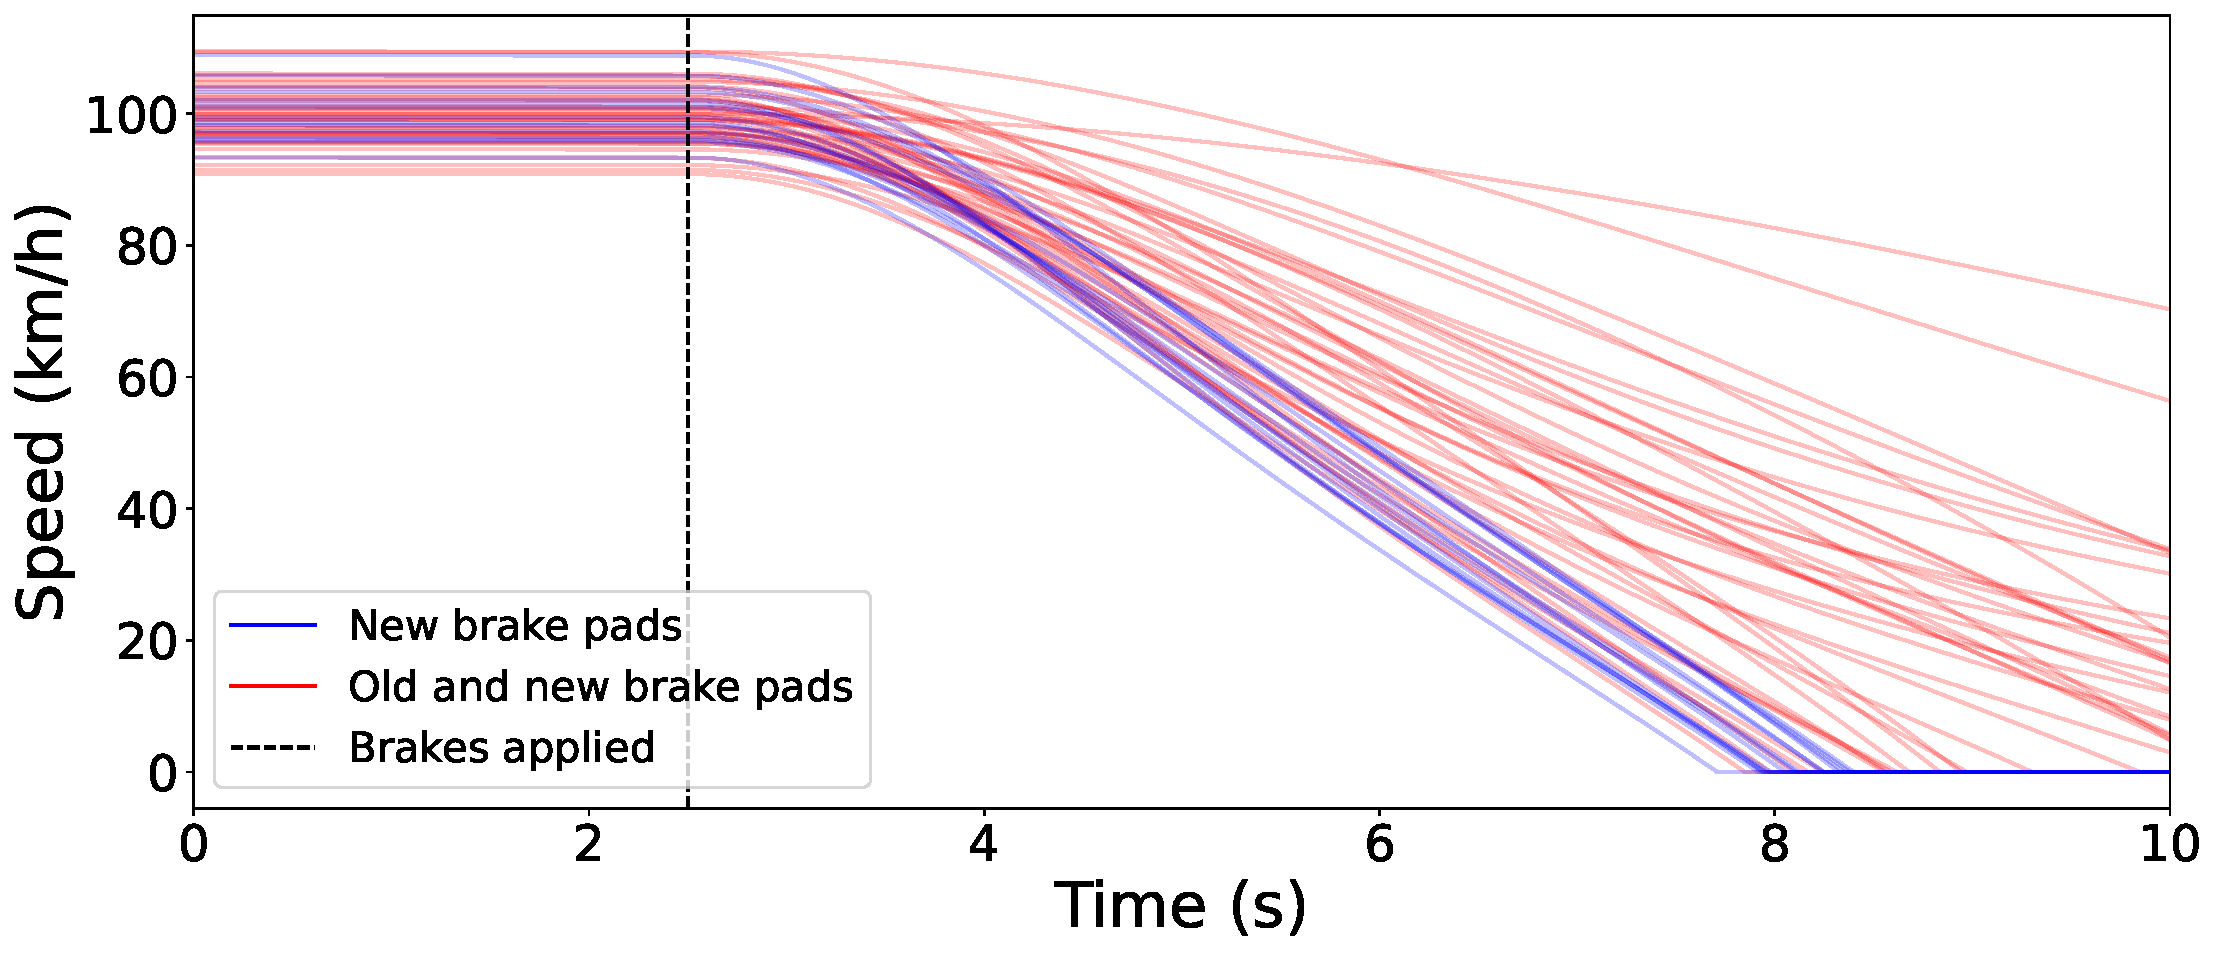
\includegraphics[height=5cm]{figures/causal/synthetic_example_newest2_nogray.pdf}
    %
    %
    %
    %

    \caption{The discrepancy between observational data and interventional behavior. The data only show the effect of aggressive braking on cars with new brake pads (blue). This differs from what \emph{would} be observed if aggressive braking were applied to the entire fleet of cars, encompassing both those with old and new brake pads (red).}
    
    %
    \label{fig:syn_ex}
\end{figure}

In the causal inference literature, any unmeasured quantity (e.g.\ brake pad age) that affects both some choice of action taken in the data (e.g.\ aggressive braking) and the resulting observation (e.g.\ speed) is referred to as an \emph{unmeasured confounder}.
In general, whenever an unmeasured confounder is present, a potential discrepancy arises between how the real-world process was observed to behave in the dataset and how it \emph{would} behave under certain interventions.
An obvious approach towards mitigating this possibility is to measure additional quantities that may affect the outcome of interest.
For example, if brake pad age were included in the data in the scenario above, then it would be possible to adjust for its effect on braking performance. 
However, in many cases, gathering additional data may be costly or impractical.
Moreover, even if this strategy is pursued, it is rarely possible to rule out the possibility of unmeasured confounding altogether, especially for complicated real-world problems \citep{tsiatis2019dynamic}. 
For example, in the scenario above, it is very conceivable that some other factor such as weather conditions could play a similar confounding role as brake pad age, and so would need also to be included in the data, and so on.
Analogous scenarios are also easily forthcoming for other application domains such as medicine and economics \citep{manski1995identification,tsiatis2019dynamic,hernan2020causal}.
%
As such, rather than attempting to sidestep the issue of unmeasured confounding, we instead propose a methodology for assessing twins using data that is robust to its presence. %

%
%
%
%
%




\section{Causal formulation} \label{sec:causal-formulation}

\subsection{The real-world process}

We begin by providing a causal model the real-world process that the twin is designed to simulate.
We do so in the language of \emph{potential outcomes} \citep{rubin1974estimating,rubin2005causal}, although we note that we could have used the alternative framework of directed acyclic graphs and structural causal models \citep{pearl2009causality} (see also \cite{imbens2020potential} for a comparison of the two).
% To streamline our presentation, we eschew certain mathematical details in the main text, especially relating to measure theory; however, the \AppendixName includes precise statements of all definitions and results that we mention.
We assume the real-world process operates over a fixed time horizon $\T \in \{1, 2, \ldots\}$.
This simplifies our presentation in what follows, and it is straightforward to generalize our methodology to variable length time horizons if needed.
For each $\tx \in \{0, \ldots, \T\}$, we assume the process gives rise to an \emph{observation} at time $\tx$, which takes values in some real-valued space $\Xspace_\tx \coloneqq \R^{\Xspacedim_\tx}$.
% standard Borel space $\Xspace_\tx$. %, and which is allowed to be multidimensional to encode multiple relevant features. % rather than only a single measurement.
We also assume that the process can be influenced by some \emph{action} taken at each time $\tx \in \{1, \ldots, \T\}$.
We denote the space of actions available at time $\tx$ by $\Aspace_\tx$, which in this work we assume is always finite.
For example, in a robotics context, the observations may consist of all the readings of all the sensors of the robot, and the actions may consist of commands that can be input by an external user.
In a medical context, the observations may consist of the vital signs of a patient, and the actions may consist of possible treatments or interventions.
To streamline notation, we will index these spaces using vector notation, so that e.g.\ $\Aspace_{1:\tx}$ denotes the cartesian product $\Aspace_1 \times \cdots \times \Aspace_\tx$, and $\ax_{1:\tx} \in \Aspace_{1:\tx}$ is a choice of $\ax_1 \in \Aspace_1, \ldots, \ax_\tx \in \Aspace_\tx$.

We model the dynamics of the real-world process via the longitudinal potential outcomes framework proposed by \cite{robins1986new}, which imposes only a weak temporal structure on the underlying phenomena of interest and so may be applied across a wide range of applications in practice.
In particular, for each $\ax_{1:\T} \in \Aspace_{1:\T}$, we posit the existence of random variables or \emph{potential outcomes} $\X_0, \X_1(\ax_1), \ldots, \X_\T(\ax_{1:\T})$, where $\X_\tx(\ax_{1:\tx})$ takes values in $\Xspace_\tx$.
We will denote this sequence more concisely as $\X_{0:\T}(\ax_{1:\T})$.
% Each $\X_\tx(\ax_{1:\tx})$ is referred to as a \emph{potential outcome}.
Intuitively, $\X_0$ represents data available before the first action, while $\X_{1:\T}(\ax_{1:\T})$ represents the sequence of real-world outcomes that \emph{would} occur if actions $\ax_{1:\T}$ were taken successively.
These quantities are therefore of fundamental interest for planning a course of actions to achieve some desired result.

% , since it determines how actions should be chosen to achieve a sequence of outcomes with optimal utility.

As random variables, each $\X_{\tx}(\ax_{1:\tx})$ may depend on additional randomness that is not explicitly modelled, and so in particular may be influenced by all the previous potential outcomes $\X_{0:\tx-1}(\ax_{1:\tx-1})$, and possibly other random quantities.
This models a process whose initial state is determined by external factors, such as when a patient from some population first presents at a hospital, and where the process then evolves according to specific actions chosen from $\Aspace_{1:\T}$ as well as additional external factors.
It is clear that this structure applies to a wide range of phenomena occurring in practice.

% and may be thought of as the counterpart of the $\xx_0$ values in each potential outcome for the twin, which represent a specific initialisation of the twin that is input deterministically by a user.


\subsection{The digital twin}

We think of the twin as a computational device that, when executed, outputs a sequence of values intended to simulate a possible future trajectory of the real-world process when certain actions in $\Aspace_{1:\T}$ are chosen, conditional on some initial data in $\Xspace_0$.
We allow the twin to make use of an internal random number generator to produce outputs that vary stochastically even under fixed inputs (although our framework encompasses twins that evolve deterministically also).
By executing the twin repeatedly, a user may therefore estimate the range of behaviours that the real-world process may exhibit under different action sequences, which can then inform planning and decision-making downstream.

Precisely, we model the output the twin would produce at timestep $\tx \in \{1, \ldots, \T\}$ after receiving initialisation $\xx_0 \in \Xspace_0$ and successive inputs $\ax_{1:\tx} \in \Aspace_{1:\tx}$ as the quantity $\twinfunction_\tx(\xx_0, \ax_{1:\tx}, \twinnoise_{1:\tx})$, where $\twinfunction_\tx$ is a measurable function taking values in $\Xspace_{\tx}$, and each $\twinnoise_\sx$ is some (possibly vector-valued) random variable.
We will denote $\Xt_{\tx}(\xx_0, \ax_{1:\tx}) \coloneqq \twinfunction_\tx(\xx_0, \ax_{1:\tx}, \twinnoise_{1:\tx})$, which we also refer to as a potential outcome.
% This means the output produced by the twin over a single trajectory may be written as
% This means a full output trajectory may be written as
A full twin trajectory therefore consists of $\Xt_1(\xx_0, \ax_1), \ldots, \Xt_\T(\xx_0, \ax_{1:\T})$, which we write more compactly by $\Xt_{1:\T}(\xx_0, \ax_{1:\T})$.
% Conceptually, $\twinfunction_\tx$ may be thought of as the program that executes inside the twin up to the point it produces its output at time $\tx$, and $\twinnoise_{1:\tx}$ may be thought of as the collection of all outputs of the internal random number generator used by the twin in order to produce this output.
Conceptually, $\twinfunction_1, \ldots, \twinfunction_\T$ constitute the program that executes inside the twin, and $\twinnoise_{1:\T}$ may be thought of as the collection of all outputs of the internal random number generator that the twin uses.
% We will assume $\twinnoise_{1:\T} \ci (\X_{0:\T}(\ax_{1:\T}) : \ax_{1:\T} \in \Aspace_{1:\T})$, i.e.\ these random number generator outputs are independent of not interact with the real-world process, which is very reasonable in practice.
We assume these random numbers $\twinnoise_{1:\T}$ and the real-world outcomes $(\X_{0:\T}(\ax_{1:\T}) : \ax_{1:\T} \in \Aspace_{1:\T})$ are independent, which is mild in practice.
We also assume that repeated executions of the twin give rise to i.i.d.\ copies of $\twinnoise_{1:\T}$.
This means that, given fixed inputs $\xx_0$ and $\ax_{1:\T}$, repeated executions of the twin produce i.i.d.\ copies of $\Xt_{1:\T}(\xx_0, \ax_{1:\T})$.
Otherwise, we make no assumptions about the precise form of either the $\twinfunction_\tx$ or the $\twinnoise_\tx$, which allows our model to encompass a wide variety of possible twin implementations.


\subsection{Correctness}

% The purpose of the twin is to predict the future of the real-world process under different possible sequences of actions.
% As such, we will assume that the twin has been designed to be correct in the following precise sense:
Before we can consider how to assess the twin, we must first define how we want the twin ideally to behave.
The following condition seems appropriate for many applications.

% We assume this is as follows.
% We assume the twin has been designed to be correct in the following sense:
% the following condition seems highly desirable for a twin in this context:


\begin{definition}[Correctness] \label{eq:interventional-correctness}
    The twin is \emph{interventionally correct} if, for $\Law[\X_0]$-almost all $\xx_0$ and $\ax_{1:\T} \in \Aspace_{1:\T}$, distribution of $\Xt_{1:\T}(\xx_0, {\ax}_{1:\T})$ is equal to the conditional distribution of $\X_{1:\T}(\ax_{1:\T})$ given $\X_0 = \xx_0$.
    % \footnote{More generally we could allow for the conditional distributions to differ byinequality up to some specified tolerance level. Additionally, as discussed in Section \rob{ref} of the Supplement, we are glossing over some technical details that arise in the general case when conditioning on events with probability zero (Section \rob{ref} of the Supplement includes a more careful discussion). However, our simplified definition here is pedagogically more useful, and suffices to convey the main ideas in what follows.
    % }
\end{definition}

% More generally we could define a notion of correctness up to some specified tolerance level.
% However, our stricter condition here is simpler, and suffices to convey the main ideas in what follows.

Operationally, if a twin is interventionally correct, then by repeatedly executing the twin and applying Monte Carlo techniques, it is possible to approximate arbitrarily well the conditional distribution of the future of the real-world process under each possible choice of action sequence.
The same can also be shown to hold when each action at each time $\tx$ is chosen dynamically on the basis of previous observations in $\Xspace_{0:\tx}$. %\footnote{We refer to Chapter 5 of \cite{tsiatis2019dynamic} for more details about how dynamically chosen interventions can be modelled within the potential outcomes framework.}
As a result, an interventionally correct twin may be used for \emph{planning}, or in other words may be used to select a policy for choosing actions that will yield a desirable distribution over observations at each step.
% the twin may be used to approximate the conditional distribution of the future of the real-world process under different choices of actions by applying Monte Carlo techniques to the outputs produced from repeated executions.
We emphasise that interventional correctness does not mean the twin will accurately predict the behaviour of any \emph{specific} trajectory of the real-world process in an almost sure sense (unless the real-world process is deterministic), but only the distribution of outcomes that will be observed over repeated independent trajectories.
However, this is sufficient for many applications, and appears to be the strongest guarantee possible when dealing with real-world phenomena whose underlying behaviour is stochastic.

Definition \ref{eq:interventional-correctness} introduces some technical difficulties that arise in the general case when conditioning on events with probability zero (e.g.\ $\{\X_0 = \xx_0\}$ if $\X_0$ is continuous).
In what follows, it is more convenient to consider an unconditional formulation of interventional correctness.
This is supplied by the following result, which considers the behaviour of the twin when it is initialised with the (random) value of $\X_0$ taken from the real-world process, rather than with a fixed choice of $\xx_0$.
See Section \ref{sec:unconditional-interventional-correctness-proof} of the \AppendixName for a proof.

% It is reasonable to make an additional structural assumption about the twin.
% In particular, we will assume that, for some function $\twinfunction$ and random variable $\twinnoise$ such that
% \begin{equation} \label{eq:random-numbers-are-independent}
%     \twinnoise \ci \{\X_{0:\T}(\ax_{1:\T}) : \ax_{1:\T} \in \Aspace_{1:\T}\},
% \end{equation}
% the potential outcomes of the twin can be expressed as follows:
% \begin{equation} \label{eq:twin-potential-outcomes-structure}
%     \Xt_{1:\T}(\xx_0, \ax_{1:\T}) = \twinfunction(\xx_0, \ax_{1:\T}, \twinnoise).
% \end{equation}
% Conceptually, $\twinfunction$ may be thought of as the program executing inside the twin, and $\twinnoise$ may be thought of as the collection of all outputs of the internal random number generator used by the twin.
% The independence assumption in \eqref{eq:random-numbers-are-independent} amounts to saying that this random number generator does not interact with the outside world, which is reasonable in practice.
% Under these assumptions, it is possible to express interventional correctness in the following equivalent way, which is more mathematically convenient in what follows:

\begin{proposition} \label{prop:interventional-correctness-alternative-characterisation}
    The twin is interventionally correct if and only if, for all choices of $\ax_{1:\T} \in \Aspace_{1:\T}$, the distribution of $(\X_0, \Xt_{1:\T}(\X_0, \ax_{1:\T}))$ is equal to the distribution of $\X_{0:\T}(\ax_{1:\T})$.
\end{proposition}


% In practice, it is reasonable to assume that the potential outcomes $\X_{0:\T}(\ax_{1:\T})$ of the real-world process are statistically independent of the potential outcomes $\Xt_{1:\T}(\xx_{0}, \ax_{1:\T})$ of the twin, or more precisely that
% \begin{equation} \label{eq:real-world-vs-twin-independence-assumption}
%     \X_0 \ci \{\Xt_{1:\T}(\xx_0, \ax_{1:\T}) : \xx_0 \in \Xspace_0, \ax_{1:\T} \in \Aspace_{1:\T}\}.
% \end{equation}
% This in effect amounts to saying that, given fixed inputs, the outputs of the twin depend only on its internal processes, and are not affected by the outside world.
% Under this assumption, it is possible to express interventional correctness in the following equivalent way, which is more mathematically convenient in what follows:

% \begin{proposition} \label{prop:interventional-correctness-alternative-characterisation}
% If \eqref{eq:real-world-vs-twin-independence-assumption} holds, then the twin is interventionally correct if and only if, for all $\ax_{1:\T} \in \Aspace_{1:\T}$, the distribution of $(\X_0, \Xt_{1:\T}(\X_0, \ax_{1:\T}))$ is equal to the distribution of $\X_{0:\T}(\ax_{1:\T})$. \faaiz{Proof}
% \end{proposition}

\subsection{Online prediction}

Our model here represents a twin at time $\tx = 0$ making predictions about all future timesteps $\tx \in \{1, \ldots, \T\}$ under different choices of inputs $\ax_{1:\T}$.
In practice, many twins are designed to receive new information at each timestep in an online fashion and update their predictions for subsequent timesteps accordingly \citep{grieves2017digital,niederer2021scaling}.
% Depending on how the twin will be deployed, various notions of correctness can be devised for this online setting.
Various notions of correctness can be devised for this online setting.
We describe two possibilities in Section \ref{sec:online-prediction} of the \AppendixName, and show that these notions of correctness essentially reduce to Definition \ref{eq:interventional-correctness}, which motivates our focus on that notion in what follows.
% , in these cases, the task of assessing correctness in the online regime essentially reduces to that of assessing correctness in the sense of Definition \ref{eq:interventional-correctness}.
% This motivates our focus on this notion in what follows.

\section{Data-driven twin assessment} \label{sec:data-driven-twin-assessment}

\subsection{Overall setup}

% We now consider how to assess the accuracy of a twin.
There are many conceivable methods for assessing the accuracy of a twin, including static analysis of the twin's source code and the solicitation of domain expertise, and in practice it seems most robust to use a combination of different techniques rather than relying on any single one \citep{amse2018assessing,niederer2021scaling}.
However, in this paper, we focus on what we will call \emph{data-driven assessment}, which we see as an important component of a larger assessment pipeline. %\footnote{For example, data-driven assessment falls naturally within the ``validation'' component of the Verification, Validation, and Uncertainty Quantification (VVUQ) framework \cite{roy2011comprehensive}.}
That is, we consider the use of statistical methods that rely solely on a dataset of trajectories obtained from the real-world process and the twin.
% We do not assume knowledge of the dynamics of the real-world process, or of the internal implementation details of the twin.
% 
% We would like to obtain a methodology that is general-purpose and can be applied to many types of datasets with confidence in its validity.
% applied to all twins for which our causal model above is appropriate.
% In particular, we want to avoid making assumptions about the real-world process, the dataset, and the internal implementation details of the twin.
% To this end, we consider a deliberately general model for how our real-world data are obtained, which we describe below.
% Our goal is to obtain a general-purpose methodology that can be applied in all contexts where our causal model above is appropriate.
% As such, we consider a deliberately very weak model for how our real-world data are obtained, which we describe below.
We show in this section that without further assumptions, it is not possible to obtain a data-driven assessment procedure that can \emph{certify} that a twin is interventionally correct.
% We show that, without adding further assumptions, 
We instead propose a strategy based on \emph{falsifying} the twin, which we develop into a concrete statistical testing procedure in later sections.

% methodology that is so that it can be applied across a wide variety of 

% We do not assume knowledge about the dynamics of the real-world process, nor access to the implementation details of the twin.

We will assume access to a dataset of trajectories obtained by observing the interaction of some behavioural agents with the real-world process.
We model each trajectory as follows.
First, we represent the action chosen by the agent at time $\tx \in \{1, \ldots, \T\}$ as an $\Aspace_\tx$-valued random variable $\A_\tx$.
We then obtain a trajectory in our dataset by recording at each step the action $\A_\tx$ chosen and the observation $\X_\tx(\A_{1:\tx})$ corresponding to this choice of action.
% as well as the specific potential outcomes $\X_\tx(\A_{1:\tx})$ corresponding to the actions chosen by the behavioural agent.
As a result, each observed trajectory has the following form:
\begin{equation} \label{eq:observed-data-trajectory}
    \X_0, \A_1, \X_1(\A_1), \ldots, \A_\T, \X_\T(\A_{1:\T}).
\end{equation}
This corresponds to the standard \emph{consistency} assumption in causal inference \citep{hernan2020causal}, and intuitively means that the potential outcome $\X_\tx(\ax_{1:\tx})$ is observed in the data when the agent actually chose $\A_{1:\tx} = \ax_{1:\tx}$.
% This corresponds to the usual \emph{stable unit treatment value assumption (SUTVA)} \cite{rubin1980randomization} (also referred to as \emph{consistency} or \emph{stability}) of the potential outcomes framework.
% SUTVA is a standard and mild assumption used to relate the interventional behaviour of the real-world process under potentially hypothetical choices of actions $\ax_{1:\tx} \in \Aspace_{1:\tx}$ to the data actually observed under the actions $\A_{1:\tx}$ actually taken.
We model our full dataset as a set of i.i.d.\ copies of \eqref{eq:observed-data-trajectory}. %, so that the observed trajectories are assumed to be mutually independent and to have the same distribution as the trajectory in \eqref{eq:observed-data-trajectory}.

% As with the real-world process and the twin, by modelling the agent's actions as random variables, we implicitly allow their value to depend on additional random quantities than we have defined here, possibly including unmeasured confounders. %, including quantities that also influence the values of potential outcomes $\X_{\tx}(\ax_{1:\tx})$.
% This leads to fundamental challenges for twin assessment that we discuss below.
% % This introduces the possibility that the the data are confounded, which leads to significant challenges for twin assessment discussed below.

% \subsection{The impossibility of verification in general}\label{sec:impossibility_of_verification}
% \paragraph{Certification strategies}
% \subsection{The impossibility of certifying that a twin is correct}\label{sec:impossibility_of_verification}

\subsection{Certification is unsound in general}

% A natural approach to twin assessment, which appears at least in principle to underlie many approaches used in practice, has the following structure.
A natural high-level strategy for twin assessment has the following structure.
First, some hypothesis $\Hyp$ is chosen with the following property:
% At a high level, these approaches first choose some hypothesis $\Hyp$ with the following property:
 \begin{equation} \label{eq:verification-hypothesis-property}
    \text{If $\Hyp$ is true, then the twin is interventionally correct.}%\footnote{More generally, and in practice more typically, we could consider a family of hypotheses that each imply correctness up to some tolerance level. However, \eqref{eq:verification-hypothesis-property} suffices for our exposition here.}
\end{equation}
% They then use the data to try to show that $\Hyp$ is true, perhaps up to some level of confidence to account for the fact that the dataset is finite.
Data is then used to try to show $\Hyp$ is true, perhaps up to some level of confidence. % to account for the fact that the dataset is finite.
If successful, it follows by construction that the twin is interventionally correct.
Assessment procedures designed to \emph{certify} the twin in this way are appealing because they promise a strong guarantee of accuracy for certified twins. % when successful.
% with this structure are appealing because they holds the promise of a strong guarantee about the accuracy of the twin.
Unfortunately, the following foundational result from the causal inference literature (often referred to as the \emph{fundamental problem of causal inference} \citep{holland1986statistics}) means that data-driven certification procedures of this kind are in general unsound, as we explain next.
For completeness, Section \ref{sec:non-identifiability-result-proof-supp} of the \AppendixName includes a self-contained proof of this result in our notation.

% We include a self-contained proof of Proposition \ref{prop:nonidentifiability} in for completeness.

% it is in general not possible to obtain a valid data-driven procedure of this kind:

% \begin{proposition} \label{prop:nonidentifiability}
%     If $\ax_{1:\T} \in \Aspace_{1:\T}$ has $\Prob(\A_{1:\T} \neq \ax_{1:\T}) > 0$, then the distribution of $\X_{0:\T}(\ax_{1:\T})$ cannot be uniquely determined from the distribution of the data in \eqref{eq:observed-data-trajectory}.
% \end{proposition}

\begin{theorem} \label{prop:nonidentifiability}
    % If $\Prob(\A_{1:\tx} \neq \ax_{1:\tx}) > 0$, then the distribution of $\X_{\tx}(\ax_{1:\tx})$ cannot be uniquely determined from the distribution of the data in \eqref{eq:observed-data-trajectory} without further assumptions.
    If $\Prob(\A_{1:\T} \neq \ax_{1:\T}) > 0$, then the distribution of $\X_{0:\T}(\ax_{1:\T})$ is not uniquely identified by the distribution of the data in \eqref{eq:observed-data-trajectory} without further assumptions.
\end{theorem}

% \noindent
% Proposition \ref{prop:nonidentifiability} is a foundational result in the causal inference literature.
% The statement holds due to what has been referred to as the \emph{fundamental problem of causal inference} \cite{holland1986statistics}, which is namely that the potential outcomes $\X_{\tx}(\ax_{1:\tx})$ are only observed in \eqref{eq:observed-data-trajectory} when $\A_{1:\tx} = \ax_{1:\tx}$.
% As such, the behaviour of the data in \eqref{eq:observed-data-trajectory} only identifies the behaviour of $\X_{\tx}(\ax_{1:\tx})$ on the event $\{\A_{1:\tx} = \ax_{1:\tx}\}$.
% On the event $\{\A_{1:\tx} \neq \ax_{1:\tx}\}$, $\X_{\tx}(\ax_{1:\tx})$ may vary arbitrarily while still giving rise to the same distribution over observational datasets.
% % In practice, it is usually very reasonable to assume that $\{\A_{1:\tx} \neq \ax_{1:\tx}\}$ occurs with positive probability, since this is only violated in the extreme case that the agent always chooses the same action sequence $\ax_{1:\tx}$.
% % In practice, $\A_{1:\tx} \neq \ax_{1:\tx}$ almost always has positive probability, since this is only violated in the extreme case that the agent always chooses the same action sequence $\ax_{1:\tx}$.
% We include a self-contained proof of Proposition \ref{prop:nonidentifiability} in Section \ref{sec:non-identifiability-result-proof-supp} of the \AppendixName for completeness.

Since the distribution of the data encodes the information that would be contained in an infinitely large dataset of trajectories, Theorem \ref{prop:nonidentifiability} imposes a fundamental limit on what can be learned about the distribution of $\X_{0:\T}(\ax_{1:\T})$ from the data we have assumed.
% Proposition \ref{prop:nonidentifiability} therefore says that, even given access to infinite data, it is not possible to identify the interventional distribution \rob{Define earlier} of the real-world process.
It follows that if $\Hyp$ is any hypothesis satisfying \eqref{eq:verification-hypothesis-property}, then $\Hyp$ cannot be determined to be true from even an infinitely large dataset.
This is because, if we could do so, then we could also determine the distribution of $\X_{0:\T}(\ax_{1:\T})$, since by Proposition \ref{prop:interventional-correctness-alternative-characterisation} this would be equal to the distribution of $(\X_0, \Xt_{\T}(\X_0, \ax_{1:\T}))$.
In other words, we cannot use the data alone to certify that the twin is interventionally correct.


\subsection{The assumption of no unmeasured confounding} \label{sec:no-unmeasured-confounding-assumption}

Theorem \ref{prop:nonidentifiability} is true in the general case, when no additional assumptions about the data-generating process are made.
One way forward is therefore to introduce assumptions under which the distribution of $\X_{0:\T}(\ax_{1:\T})$ \emph{can} be identified.
This would mean it is possible to certify that the twin is interventionally correct, since, at least in principle, we could simply check whether this matches the distribution of $(\X_0, \Xt_{1:\T}(\X_{0}, \ax_{1:\T}))$ produced by the twin.

The most common such assumption in the causal inference literature is that the data are free of \emph{unmeasured confounding}.
Informally, this holds when each action $\A_\tx$ is chosen by the behavioural agent solely on the basis of the information available at time $\tx$ that is actually recorded in the dataset, namely $\X_{0}, \A_1, \X_1(\A_1), \ldots, \A_{\tx-1}, \X_{\tx-1}(\A_{1:\tx-1})$, as well as possibly some additional randomness that is independent of the real-world process, such as the outcome of a coin toss. (This can be made precise via the \emph{sequential randomisation assumption} introduced by \cite{robins1986new}.)
% \footnote{ Chapter 5 of \cite{tsiatis2019dynamic} provides an overview of this.}
% \footnote{Formally, the data are unconfounded when $\A_\tx \ci \{\X_{\sx}(\ax_{1:\sx}) : \sx \geq \tx, \ax_{1:\sx} \in \Aspace_{1:\sx}\} \mid \X_{0:\tx-1}(\A_{1:\tx-1}), \A_{1:\tx-1}$ for all $\tx \in \{1, 2, \ldots\}$ \cite{robins1986new}.}
Unobserved confounding is present whenever this does not hold, i.e.\ whenever some unmeasured factor simultaneously influences both the agent's choice of action and the observation produced by the real-world process.
% For instance, in the motivating example given in Section \ref{sec:motivating-example}, brake pad age is an unobserved confounder since it affects both the decision to brake aggressively, as well as the resulting speed of the car.

It is reasonable to assume that the data are unconfounded in certain contexts.
For example, in certain situations it may be possible to gather data in a way that specifically guarantees there is no confounding.
Randomised controlled trials, which ensure that each $\A_\tx$ is chosen via a carefully designed randomisation procedure \citep{lavori2004dynamic,murphy2005experimental}, constitute a widespread example of this approach.
Likewise, it is possible to show that the data are unconfounded if each $\X_\tx(\ax_{1:\tx})$ is a deterministic function of $\X_{0:\tx-1}(\ax_{1:\tx-1})$ and $\ax_{\tx}$, which may be reasonable to assume for example in certain low-level physics or engineering contexts.
(See Section \ref{eq:deterministic-potential-outcomes-are-unconfounded} of the \AppendixName for a proof.)
However, for stochastic phenomena and for typical datasets, it is widely acknowledged that the assumption of no unmeasured confounding will rarely hold, and so assessment procedures based on this assumption may yield unreliable results in practice \citep{murphy2003optimal,tsiatis2019dynamic}.
Section \ref{sec:motivating-example} of the \AppendixName illustrates this concretely with a toy scenario.
% describes a simple scenario , and illustrates how naive approaches for twin assessment may be misleading.
% the pitfalls that may result from naive approach to twin assessment.

% However, for general datasets, where no such care has necessarily been taken, this assumption seems highly tenuous. \rob{Cite Tsiatis}
% As a result, verification procedures that rely on this assumption may yield unreliable results in practice.


\subsection{General-purpose assessment via falsification}

Our goal is to obtain an assessment methodology that is general-purpose, and as such we would like to avoid introducing assumptions such as unconfoundedness that do not hold in general.
% To achieve this, motivated by the philosophical work of Popper, we propose a strategy that replaces the goal of verifying the interventional correctness of the twin with that of falsifying it \cite{popper2005logic}.
To achieve this, borrowing philosophically from \cite{popper2005logic}, we propose a strategy that replaces the goal of verifying the interventional correctness of the twin with that of \emph{falsifying} it.
Specifically, we consider hypotheses $\Hyp$ with the dual property to \eqref{eq:verification-hypothesis-property}, namely:
\begin{equation} \label{eq:falsification-hypothesis-property}
    \text{If the twin is interventionally correct, then $\Hyp$ is true.}
\end{equation}
We will then try to show that each such $\Hyp$ is \emph{false}.
% For each such $\Hyp$, we will try to show that $\Hyp$ is false.
Whenever we are successful, we will thereby have gained some knowledge about a failure mode of the twin, since by construction the twin can only be correct if $\Hyp$ is true.
In effect, each $\Hyp$ we falsify will constitute a \emph{reason} that the twin is not correct, and may suggest concrete improvements to its design, or may identify cases where its output should not be trusted.

Importantly, unlike for \eqref{eq:verification-hypothesis-property}, Theorem \ref{prop:nonidentifiability} does not preclude the possibility of data-driven assessment procedures based on \eqref{eq:falsification-hypothesis-property}.
As we show below, there do exist hypotheses $\Hyp$ satisfying \eqref{eq:falsification-hypothesis-property} that can in principle be determined to be false from the data alone without additional assumptions.
In this sense, falsification provides a means for \emph{sound} data-driven twin assessment, %and falsification-based approaches may constitute a useful addition to existing twin assessment pipelines in safety-critical settings where robustness and reliability are essential.
whose results can be relied upon across a wide range of circumstances.
On the other hand, falsification approaches cannot provide a \emph{complete} guarantee about the accuracy of a twin: even if we fail to falsify many $\Hyp$ satisfying \eqref{eq:falsification-hypothesis-property}, we cannot then infer that the twin is correct.
As such, in situations where (for example) it is reasonable to believe that the data are in fact unconfounded, it may be desirable to use this assumption to obtain additional information about the twin than is possible from falsification alone.
% to try to show that the twin is interventionally correct.


% Overall, our approach follows the guidelines for empirical analysis proposed by econometrician Charles Manski \cite{manski1995identification}, who advocates for researchers always to establish a ``domain of consensus'' \cite{manski2009identification} by analysing their data initially under minimal assumptions, and only afterwards to consider what follows as assumptions of various strengths are introduced.
% To this end, Manski and others developed a literature on \emph{partial identification} \cite{manski1989anatomy,manski,balke1997bounds,manski1997monotone,manski2000monotone,manski2003partial,imbens2004confidence,chernozhukov2007estimation} to provide precise statistical tools with which this high-level strategy may be implemented.
% Similar ideas and motivations have also appeared in more recent work \cite{bareinboim,murphy2003optimal,hussain2022falsification}.
% % to analyse their data under minimal assumptions so as to establish an initial ``domain of consensus'' \cite{manski2009identification}, and only afterwards to consider what follows as assumptions of various strengths are introduced.
% Using ideas from this literature, in Sections \ref{sec:hypotheses-from-causal-bounds} and \ref{sec:statistical-methodology} below we propose a twin assessment procedure based on falsification that leads to granular quantitative information about the twin that could be used in downstream tasks.
% % In the next section, we use ideas from this literature give rise to a family of $\Hyp$ satisfying \eqref{eq:falsification-hypothesis-property} whose falsification leads to granular quantitative information about the twin that could be used downstream.
% % We then provide a statistical testing procedure that can be used to falsify these hypotheses using a finite dataset.
% Our methodology requires no additional assumptions beyond those already described, and so is % be applied confidently across a wide variety of possible twins and datasets.
% suitable for twin assessment pipelines in safety-critical settings where robustness is essential.

% Overall, our approach follows the guidelines for empirical analysis proposed by econometrician Charles Manski \cite{manski1995identification}, who advocates for researchers always to establish a ``domain of consensus'' \cite{manski2009identification} by analysing their data initially under minimal assumptions, and only afterwards to consider what follows as assumptions of various strengths are introduced.
% To this end, Manski and others developed a literature on \emph{partial identification} of probability distributions \cite{manski1989anatomy,manski,balke1997bounds,manski1997monotone,manski2000monotone,manski2003partial,imbens2004confidence,chernozhukov2007estimation} in order to provide precise statistical tools with which this high-level strategy may be implemented.
% Similar ideas and motivations have appeared in more recent work: notably, \cite{bareinboim} use partial identification techniques to obtain a more efficient algorithm for the online learning of optimal dynamic treatment regimes \cite{murphy2003optimal}, while \cite{hussain2022falsification} propose a meta-algorithm that involves falsifying treatment effect estimators that can be determined to be invalid using data from a randomised controlled trial.
% % to analyse their data under minimal assumptions so as to establish an initial ``domain of consensus'' \cite{manski2009identification}, and only afterwards to consider what follows as assumptions of various strengths are introduced.
% In the next section, we describe how ideas from this literature give rise to a family of $\Hyp$ satisfying \eqref{eq:falsification-hypothesis-property} whose falsification leads to granular quantitative information about the twin that could be used downstream.
% We then provide a statistical testing procedure that can be used to falsify these hypotheses using a finite dataset.
% Our resulting methodology requires no additional assumptions beyond those already described, and so may % be applied confidently across a wide variety of possible twins and datasets.
% constitute a valuable addition to twin assessment pipelines in safety-critical settings where robustness is essential.


% In the next section we describe how ideas from the literature on partial identification of probability distributions -- which was initiated by Manski to this end \cite{manski2003partial} -- may be used to obtain a concrete methodology for falsifying a twin without the requirement of any further modelling assumptions.
% 
% a family of causal bounds whose development began with Manski may be used to obtain a concrete methodology for falsifying a twin without the requirement of any further modelling assumptions.
% While the assessment procedure we obtain cannot provide \emph{complete} information about the accuracy of the twin, its outputs are accompanied by strong statistical guarantees of \emph{soundness}, and so our proposal (and falsification procedures more generally) may constitute an important addition to existing twin assessment pipelines in safety-critical settings where robustness and reliability are essential.


% % may constitute an important addition to existing twin assessment pipelines across a wide variety of applications.

% Given the safety-critical nature of the application domains of many twins, this reliability property appears highly desirable

% As such, the resulting methodology (and falsification more generally)
% may constitute an important addition to existing twin assessment pipelines across a wide variety of applications.



% \Rob{Manski's philosophy?}



\section{Longitudinal causal bounds} \label{sec:causal-bounds}

\subsection{Statement of result} \label{sec:causal-bounds-statement}

One possible means for obtaining interventional information about the twin is via the classical bounds proposed by \cite{manski}.
These bounds hold without further assumptions, and so could in principle give rise to a sound falsification procedure of the kind we are seeking.
However, although they have been successfully applied in various cases, Manski's bounds are often very conservative, and so would not lead to very informative results if used directly.
To address this, we propose a novel generalisation of these bounds that explicitly accounts for the temporal structure of our setting.
As we explain below, our bounds can become considerably more informative than those of Manski, while also not requiring the addition of untestable causal assumptions.
% they depend only on assumptions that can be tested directly using the observational data.
We provide these bounds next, along with several theoretical results about their behaviour and optimality.
In Section \ref{sec:hypotheses-from-causal-bounds}, we use these bounds to define a class of $\Hyp$ with the desired property \eqref{eq:falsification-hypothesis-property}, which then yields a procedure for falsifying twins through hypothesis testing techniques.


% \begin{itemize}
%     \item Manski's bounds are a classical result
%     \item They can be used without any further assumptions (and are the best possible in this case) 
%     \item However, they are very loose in many cases in practice
%     \item A common strategy of prior work is to introduce assumptions to avoid this
%     \item We instead exploit the temporal structure of our problem to get more informative bounds without additional assumptions
% \end{itemize}

% We now describe a novel longitudinal variant of Manski's classical bounds \citep{manski} from the causal inference literature.
% Intuitively, this result bounds the expected outcome output by any interventionally correct twin.
% In the next section, we use this result to define hypotheses $\Hyp$ with the desired property \eqref{eq:falsification-hypothesis-property}, which then yields a procedure for falsifying twins via hypothesis testing techniques.
% % Our result accounts for the longitudinal structure of our problem appropriately.
% We now describe a novel variant of a classical family of bounds from the causal inference literature whose development began with Manski \cite{manski}, and that is suited to the longitudinal nature of our problem.
% Intuitively, any twin that is interventionally correct must satisfy these bounds.
% In the next section, we use this result accordingly to define hypotheses $\Hyp$ satisfying our desired property \ref{eq:falsification-hypothesis-property}
% Our hypotheses $\Hyp$ are based on a classical family of bounds from the causal inference literature whose development began with Manski \cite{manski}.
% We derive a novel variant of these bounds that is more suited to the longitudinal nature of our problem.
% We therefore propose a novel alternative form of these bounds that is considerably simpler and for which an unbiased estimator is easily forthcoming.


\begin{theorem} \label{thm:causal-bounds}
    Suppose $(\Y(\ax_{1:\tx}) : \ax_{1:\tx} \in \Aspace_{1:\tx})$ are real-valued potential outcomes defined jointly with $(\X_{0:\T}(\ax_{1:\T}) : \ax_{1:\T} \in \Aspace_{1:\T})$ and $\A_{1:\T}$. If for some $\tx \in \{1, \ldots, \T\}$, $\ax_{1:\tx} \in \Aspace_{1:\tx}$, measurable $\B_{0:\tx} \subseteq \Xspace_{0:\tx}$, and $\ylo, \yup \in \R$ we have
%     \begin{align}
\noindent
% \begin{minipage}[b]{0.35\linewidth}
% \begin{align}
%     \Prob(\X_{0:\tx}(\ax_{1:\tx}) \in \B_{0:\tx}) &> 0 \label{eq:B-positivity-assumption}
% \end{align}
% \end{minipage}%
% \begin{minipage}[b]{0.65\linewidth}
% \begin{align}
%     \Prob(\ylo \leq \Y(\ax_{1:\tx}) \leq \yup \mid \X_{0:\tx}(\ax_{1:\tx}) \in \B_{0:\tx}) &= 1.  \label{eq:Y-boundedness-assumption}
% \end{align}
% \end{minipage}
% 
% \end{align}
    \begin{gather}
        \Prob(\X_{0:\tx}(\ax_{1:\tx}) \in \B_{0:\tx}) > 0 \label{eq:B-positivity-assumption} \\
        \Prob(\ylo \leq \Y(\ax_{1:\tx}) \leq \yup \mid \X_{0:\tx}(\ax_{1:\tx}) \in \B_{0:\tx}) = 1,  \label{eq:Y-boundedness-assumption}
    \end{gather}
    \noindent then it holds that
    \begin{equation} \label{eq:causal-bounds-fully-written}
        \E[\Ylo \mid \X_{0:\N}(\A_{1:\N}) \in \B_{0:\N}]
        \leq \E[\Y(\ax_{1:\tx}) \mid \X_{0:\tx}(\ax_{1:\tx}) \in \B_{0:\tx}]
        \leq  \E[\Yup \mid \X_{0:\N}(\A_{1:\N}) \in \B_{0:\N}],
    \end{equation}
    % where we define the following random variables \faaiz{awkward}: $\N \coloneqq \max \{0 \leq \sx \leq \tx \mid \A_{1:\sx} = \ax_{1:\sx}\}$,
    where we define $\N \coloneqq \max \{0 \leq \sx \leq \tx \mid \A_{1:\sx} = \ax_{1:\sx}\}$, and similarly
    \begin{align*}
        \Ylo \coloneqq \ind(\A_{1:\tx} &= \ax_{1:\tx}) \, \Y(\A_{1:\tx}) + \ind(\A_{1:\tx} \neq \ax_{1:\tx}) \, \ylo \\
        \Yup \coloneqq \ind(\A_{1:\tx} &= \ax_{1:\tx}) \, \Y(\A_{1:\tx}) + \ind(\A_{1:\tx} \neq \ax_{1:\tx}) \, \yup.
    \end{align*}

    %     \Qlo \coloneqq \E[\Ylo \mid \X_{0:\N}(\A_{1:\N}) \in B_{0:\N}] \qquad  \Qup \coloneqq \E[\Yup \mid \X_{0:\N}(\A_{1:\N}) \in B_{0:\N}].
    
    % we have $\Qlo \leq \Q \leq \Qup$, where $\Q \coloneqq \E[\Y(\ax_{1:\tx}) \mid \X_{0:\tx}(\ax_{1:\tx}) \in B_{0:\tx}]$,
    % \[
    %     \Qlo \coloneqq \E[\Ylo \mid \X_{0:\N}(\A_{1:\N}) \in B_{0:\N}] \qquad  \Qup \coloneqq \E[\Yup \mid \X_{0:\N}(\A_{1:\N}) \in B_{0:\N}].
    % \]
    % \[
    %     \E[\Ylo \mid \X_{0:\N}(\A_{1:\N}) \in \B_{0:\N}]
    %     \leq \E[\Y(\ax_{1:\tx}) \mid \X_{0:\tx}(\ax_{1:\tx}) \in \B_{0:\tx}]
    %     \leq \E[\Yup \mid \X_{0:\N}(\A_{1:\N}) \in \B_{0:\N}].
    % \]
\end{theorem}
(See Section \ref{sec:causal-bounds-proofs} of the \AppendixName for a proof.)

% We state the result before providing intuition below.
For brevity, in what follows we will write the terms in \eqref{eq:causal-bounds-fully-written} as $\Qlo$, $\Q$, and $\Qup$ respectively, so the conclusion of this result becomes $\Qlo \leq \Q \leq \Qup$.

Intuitively, $\Y(\ax_{1:\tx})$ here may be thought of as some quantitative outcome of interest.
For example, in a medical context, $\Y(\ax_{1:\tx})$ might represent the heart rate of a patient at time $\tx$ after receiving some treatments $\ax_{1:\tx}$.
When defining our hypotheses below, we consider the specific form $\Y(\ax_{1:\tx}) \coloneqq \fx(\X_{0:\tx}(\ax_{1:\tx}))$, where $\fx : \Xspace_{0:\tx} \to \R$ is some scalar function.
The value $\Q$ is then simply the (conditional) average behaviour of this outcome.
By Theorem \ref{prop:nonidentifiability}, $\Q$ is in general not identified by the data since it depends on $\X_{0:\tx}(\ax_{1:\tx})$.
% In general, the , is not identified by the distribution of the data \faaiz{say $\Q$ is not identifiable?}, since it depends 
% However,  
% $\Q$ depends on the distribution of $\X_{0:\tx}(\ax_{1:\tx})$, which by is not uniquely identified by
On the other hand, both $\Qlo$ and $\Qup$ \emph{are} identified, since the relevant random variables $\Ylo$, $\Yup$, $\N$, and $\X_{0:\N}(\A_{1:\N})$ can all be expressed as functions of the observed data $\X_{0:\tx}(\A_{1:\tx})$ and $\A_{1:\tx}$.
In this way, Theorem \ref{thm:causal-bounds} bounds the behaviour of a non-identifiable quantity in terms of identifiable ones.
At a high level, this is achieved by replacing $\Y(\ax_{1:\tx})$, whose value is only observed on the event $\{\A_{1:\tx} = \ax_{1:\tx}\}$, with $\Ylo$ and $\Yup$, which are equal to $\Y(\ax_{1:\tx})$ when its value is observed (i.e.\ when $\A_{1:\tx} = \ax_{1:\tx}$), and which fall back to the worst-case values of $\ylo$ and $\yup$ otherwise.
% The full details of the proof are given in the \AppendixName.
We emphasise that Theorem \ref{thm:causal-bounds} does not require any additional causal assumptions, and in particular remains true under arbitrary unmeasured confounding.

% It therefore seems reasonable to expect \eqref{eq:causal-bounds-result} will hold for a very wide variety of datasets that occur in practice.
% We also note that the theorem does not \emph{require} $\Y(\ax_{1:\tx}) = \fx(\X_{0:\tx}(\ax_{1:\tx}))$, and applies more generally to any random variables $\Y(\ax_{1:\tx})$ defined on the same probability space as our model.

% Indeed, any choice of scalar function $\fx : \Xspace_{0:\tx} \to \R$ gives rise to a choice of $\Y(\ax_{1:\tx}) \coloneqq \fx(\X_{0:\tx}(\ax_{1:\tx}))$, and this is the form we consider when defining our hypotheses from these bounds below.

In the structural causal modelling framework \citep{pearl2009causality}, a related result to Theorem \ref{thm:causal-bounds} was given as Corollary 1 by \citet{bareinboim}.
However, their result involves a complicated ratio of unknown quantities that makes estimation of their bounds difficult, since it is not obvious how to obtain an unbiased estimator for their ratio term.
% in a very different form 
% first proposed \Rob{Weaken?} as Corollary 1 of Zhang \& Bareinboim \cite{bareinboim} that is more suited to the longitudinal nature of our problem.
% However, the bounds in \cite{bareinboim} involves a complicated expression of ratios of unknown quantities that makes their statistical estimation difficult, since it is not obvious how to obtain an unbiased estimator for this ratio.
In contrast, our proposed causal bounds are considerably simpler, since both $\Qlo$ and $\Qup$ here are expressed as (conditional) expectations. 
This makes their unbiased estimation straightforward, which we use to obtain exact confidence intervals for both terms in Section \ref{sec:statistical-methodology}.

% simpler, and easily give rise to an unbiased estimator with attractive theoretical properties.

% We point out that the bounds 
% We also note that, although we do make use of it in our experiments, it is possible to obtain an alternative version of this result that conditions 



\subsection{Informativeness} \label{sec:informativeness-of-our-bounds}

For Theorem \ref{thm:causal-bounds} to be useful in practice, we would like the bounds $[\Qlo, \Qup]$ to be relatively narrower than the worst-case bounds $[\ylo, \yup]$ that are trivially implied by \eqref{eq:Y-boundedness-assumption}.
We can quantify the extent to which this occurs by the ratio
\begin{equation} \label{eq:tightness-of-bounds-measure}
    \frac{\Qup - \Qlo}{\yup - \ylo} = 1 - \Prob(\A_{1:\tx} = \ax_{1:\tx} \mid \X_{0:\N}(\A_{1:\N}) \in \B_{0:\N}),
\end{equation}
where the equality here follows from the definitions of $\Qlo$ and $\Qup$ together with some straightforward manipulations.
% Here the left-hand side quantifies the tightness of the bounds $[\Qlo, \Qup]$ relative to the worst-case bounds $[\ylo, \yup]$ that are trivially implied by \eqref{eq:Y-boundedness-assumption}, with smaller values meaning tighter bounds.
% In this way, the tightness of the bounds is determined by the value of $\Prob(\A_{1:\tx} = \ax_{1:\tx} \mid \X_{0:\N}(\A_{1:\N}) \in \B_{0:\N})$, which is closely related to the classical \emph{propensity score} in the causal inference literature \citep{rosenbaum1983central}. %, and quantifies how likely the action sequence $\ax_{1:\tx}$ is to occur in the data.
In other words, the (relative) tightness of our bounds is determined by the value of $\Prob(\A_{1:\tx} = \ax_{1:\tx} \mid \X_{0:\N}(\A_{1:\N}) \in \B_{0:\N})$, which is itself closely related to the classical \emph{propensity score} in the causal inference literature \citep{rosenbaum1983central}. %, and quantifies how likely the action sequence $\ax_{1:\tx}$ is to occur in the data.
Intuitively, as this probability grows larger, so too does $\Prob(\Y(\ax_{1:\tx}) = \Y(\A_{1:\tx}) \mid \X_{0:\N}(\A_{1:\N}) \in \B_{0:\N})$, which means the effect of unmeasured confounding on the value of $\Q$ is reduced, leading to tighter bounds.
% The bounds become looser for action sequences with a low probability of being chosen, since in this case a greater proportion of interventional outcomes $\Y(\ax_{1:\tx})$ remain unobserved.

Theorem \ref{thm:causal-bounds} is a generalisation of the bounds proposed by \cite{manski}, which can be recovered as the case where $\B_{0:\tx} = \Xspace_{0:\tx}$, so that \eqref{eq:causal-bounds-fully-written} becomes $\E[\Ylo] \leq \E[\Y(\ax_{1:\tx})] \leq \E[\Yup]$.
In practice, Manski's result is often regarded as quite uninformative.
From \eqref{eq:tightness-of-bounds-measure}, this is true whenever $\Prob(\A_{1:\tx} = \ax_{1:\tx})$ is small, which often occurs in many applications, particularly for longer action sequences.
% can be seen to occur because $\Prob(\A_{1:\tx} = \ax_{1:\tx})$ is often small in practice, especially as action sequences grow longer.
On the other hand, in many contexts it seems reasonable to anticipate that certain longer action sequences will be fairly likely to occur when conditioned on some intermediate observations.
In other words, $\Prob(\A_{1:\tx} = \ax_{1:\tx} \mid \X_{0:\N}(\A_{1:\N}) \in \B_{0:\N})$ may be large, even if $\Prob(\A_{1:\tx} = \ax_{1:\tx})$ is not.
By choosing $\B_{0:\tx}$ carefully, we can therefore obtain tighter bounds than would be possible by using Manski's original result.
The following straightforward result provides a sufficient condition for this to hold.
In Section \ref{sec:case-study} below, we also show empirically that Theorem \ref{thm:causal-bounds} yields more informative results in our case study compared with Manski's original bounds.

% We also show empirically the benefit of Theorem \ref{thm:causal-bounds} in our case study provided in Section \ref{sec:case-study} below.

% In Section \ref{sec:case-study}, we also verify empirically that Theorem \ref{thm:causal-bounds} is more informative than Manski's bounds for our application.

% hat this occurs empirically in our experiments below.

\begin{proposition} \label{prop:our-bounds-vs-manskis}
    Consider the same setup as Theorem \ref{thm:causal-bounds}, where also $\ylo \leq \Y(\ax_{1:\tx}) \leq \yup$ almost surely.
    If $\Prob(\A_{1:\tx} = \ax_{1:\tx} \mid \X_{0:\N}(\A_{1:\N}) \in \B_{0:\N}) > \Prob(\A_{1:\tx} = \ax_{1:\tx})$, then the width of Manski's bounds exceeds that of Theorem \ref{thm:causal-bounds}, i.e.\ $\E[\Yup] - \E[\Ylo] > \Qup - \Qlo$.
\end{proposition}

Beyond allowing us to obtain tighter bounds, the conditional nature of Theorem \ref{thm:causal-bounds} also appears of interest simply for its own sake.
In particular, Theorem \ref{thm:causal-bounds} describes the interventional behaviour of $\Y(\ax_{1:\tx})$ conditional on the behaviour of the trajectory $\X_{0:\tx}(\ax_{1:\tx})$, thereby providing more granular information than can be obtained from unconditional bounds of \cite{manski} alone.

% Beyond allowing us to obtain tighter bounds than those of Manski, Theorem \ref{thm:causal-bounds} intuitively also allows us to consider the interventional behaviour of the outcome for different subpopulations (denoted by $\B_{0:\tx}$). This yields more granular information than that provided by Manski. 

% allows us to obtain more granular information about the behaviour $\Y(\ax_{1:\tx})$

% By allowing $\B_{0:\tx}$ to be general, Theorem \ref{thm:causal-bounds} gives rise to more granular family of statements about the behaviour of $\Y(\ax_{1:\tx})$ than can be obtained otherwise.
% This additional granularity is of interest for its own sake, since it provides more precise information about the behaviour of the twin.


% The informativeness of the bounds in Theorem \ref{thm:causal-bounds} in practice depends on  tightness of the bounds in Theorem \ref{thm:causal-bounds}.



% \Rob{Fix this. One issue with explaining what is going on is that $\Q$ is determined by the joint behaviour of the real-world process, whereas we have only said that the conditional is not identifiable.}




% The effectiveness of the falsification procedure we describe below depends on the tightness of the bounds in \eqref{eq:causal-bounds-result}, which in turn is determined by the value of $\Prob(\A_{1:\tx} = \ax_{1:\tx} \mid \X_{0:\N}(\A_{1:\N}) \in \B_{0:\N})$.
% \rob{Should comment that when this is large, the bounds approach $\Q$}
% This value is closely related to the classical \emph{propensity score} in the causal inference literature \cite{rosenbaum1983central}, and quantifies how likely the action sequence $\ax_{1:\tx}$ is to occur in the data.
% % As the propensity approaches $1$,
% % The informativeness of these bounds depends on how close $\Prob(\A_{1:\tx} = \ax_{1:\tx} \mid \X_{0:\N}(\A_{1:\N}) \in \B_{0:\N})$ is to $1$, i.e.\ on how likely the action sequence $\ax_{1:\tx}$ is to be chosen by the behavioural agent. \rob{Refer to as ``propensity''? (Do we use this term later?)}
% % Intuitively, for very likely action sequences, the distribution of the worst-case estimates $\Ylo$ and $\Yup$ is a good approximation to the distribution of $\Y(\ax_{1:\tx})$, since $\Y(\ax_{1:\tx}) = \Y(\A_{1:\tx})$ holds with very high probability. 
% Intuitively, for very likely action sequences, $\Y(\ax_{1:\tx}) = \Y(\A_{1:\tx})$ holds with very high probability.
% This means that the effect of unmeasured confounding on the overall expectation is limited, and implies that the bounds on $\Q$ are tight.
% The bounds become looser for action sequences with a low probability of being chosen, since in this case a greater proportion of interventional outcomes $\Y(\ax_{1:\tx})$ remain unobserved.
% In the extreme case that $\A_{1:\tx} = \ax_{1:\tx}$ has zero probability of occurring, \eqref{eq:causal-bounds-result} relaxes to the worst-case bounds $[\ylo, \yup]$ that are trivially implied by \eqref{eq:Y-boundedness-assumption}.


\subsection{Optimality}

% We now consider whether the bounds in Theorem \ref{thm:causal-bounds} are in some sense optimal.
% (We consider our particular case in Sections \ref{sec:our-case-sharpness} and \ref{sec:continuous-subsequent-covariates} of the \AppendixName, drawing essentially the same conclusions as here.) \rob{Move or remove}
% % a situation that does not conform to our model but that may be of interest in other contexts.
The following result shows that Theorem \ref{thm:causal-bounds} cannot be improved without further assumptions. 
Intuitively speaking, there always exists \emph{some} family of potential outcomes that produces the same observational data as our model, but that attains the worst-case bounds $\Qlo$ or $\Qup$.
Therefore, we cannot rule out the possibility that the true potential outcomes achieve $\Qlo$ or $\Qup$ from the observational data alone.
% Therefore, given only the observational data, it is impossible for us to obtain a tighter lower bound than $\Qlo$ without making any additional assumptions. The same holds for $\Qup$ as well.
% \rob{More intuition}
% Intuitively, we cannot rule out the possibility 

\begin{proposition} \label{prop:sharpness-of-bounds}
    Under the same setup as in Theorem \ref{thm:causal-bounds}, there always exists potential outcomes $(\tilde{\X}_{0:\T}(\ax_{1:\T}'), \tilde{\Y}(\ax_{1:\tx}') : \ax_{1:\T}' \in \Aspace_{1:\T})$ also satisfying \eqref{eq:Y-boundedness-assumption} (mutatis mutandis) with 
    $$(\tilde{\X}_{0:\T}(\A_{1:\T}), \tilde{\Y}(\A_{1:\tx}), \A_{1:\T}) \eqas (\X_{0:\T}(\A_{1:\T}), \Y(\A_{1:\tx}), \A_{1:\T})$$ 
    but for which $$\E[\tilde{\Y}(\ax_{1:\tx}) \mid \tilde{\X}_{0:\tx}(\ax_{1:\tx}) \in \B_{0:\tx}] = \Qlo.$$
    The corresponding statement is also true for $\Qup$.
\end{proposition}

Apart from attempting to tighten our bounds on $\Q$, in some cases we may wish to consider bounding the alternative quantity $\E[\Y(\ax_{1:\tx}) \mid \X_{0:\tx}(\ax_{1:\tx})]$ that conditions on the \emph{value} of $\X_{0:\tx}(\ax_{1:\tx})$ rather than on the event $\{\X_{0:\tx}(\ax_{1:\tx}) \in \B_{0:\tx}\}$.
% For falsification purposes, this would provide a means for determining that twin is incorrect when it outputs specific values of $\Xt_{0:\tx}(\ax_{1:\tx})$, rather than just that it is incorrect on average across all runs that output values $\Xt_{0:\tx}(\ax_{1:\tx}) \in \B_{0:\tx}$.
To achieve this, it is natural to generalize our assumption \eqref{eq:Y-boundedness-assumption} by supposing we now have measurable functions $\ylo, \yup : \Xspace_{0:\tx} \to \R$ such that
\begin{equation} \label{eq:worst-case-behaviour-functional-assumption}
    \ylo(\X_{0:\tx}(\ax_{1:\tx})) \leq \Y(\ax_{1:\tx}) \leq \yup(\X_{0:\tx}(\ax_{1:\tx})) \qquad \qquad \text{almost surely,}
\end{equation}
and our goal is to obtain measurable functions $\lo{\gx}, \up{\gx} : \Xspace_{0:\tx} \to \R$ such that
\begin{equation} \label{eq:almost-sure-bound-desired-result}
    \lo{\gx}(\X_{0:\tx}(\ax_{1:\tx})) \leq \E[\Y(\ax_{1:\tx}) \mid \X_{0:\tx}(\ax_{1:\tx})] \leq \up{\gx}(\X_{0:\tx}(\ax_{1:\tx})) \qquad \qquad \text{almost surely.}
\end{equation}
As we describe in Section \ref{sec:impossibility-of-bounds-for-continuous-data} of the \AppendixName, bounds of this kind can be obtained directly from Theorem \ref{thm:causal-bounds} if $\X_{0:\tx}(\ax_{1:\tx})$ is discrete, or by a simple modification of the proof of Theorem \ref{thm:causal-bounds} if $\X_{1:\tx}(\ax_{1:\tx})$ is discrete (but $\X_0$ is possibly continuous).
However, somewhat surprisingly, in general we cannot obtain nontrivial bounds of this kind without further assumptions beyond the discrete case.
To make this precise, we will say that a given $\lo{\gx}$ and $\up{\gx}$ are \emph{permissible} if \eqref{eq:almost-sure-bound-desired-result} holds when $(\X_{0:\T}(\ax_{1:\tx}), \Y(\ax_{1:\tx}), \A_{1:\T} : \ax_{1:\T}' \in \Aspace_{1:\T})$ are replaced by any potential outcomes $(\tilde{\X}_{0:\T}(\ax_{1:\T}'), \tilde{\Y}(\ax_{1:\tx}'), \tilde{\A}_{1:\T} : \ax_{1:\T}' \in \Aspace_{1:\T})$  for which $\Law[\tilde{\X}_{0:\T}(\tilde{\A}_{1:\T}), \tilde{\A}_{1:\T}, \tilde{\Y}(\tilde{\A}_{1:\tx})] = \Law[\X_{0:\T}(\A_{1:\T}), \A_{1:\T}, \Y(\A_{1:\tx})]$, and which also satisfy \eqref{eq:worst-case-behaviour-functional-assumption} (mutatis mutandis).
Intuitively, this means that $\lo{\gx}$ and $\up{\gx}$ depend only on the information we have available, i.e.\ the observational distribution and our assumed worst-case values.
We then have the following:

% is \emph{compatible} with ours if it also satisfies \eqref{eq:worst-case-behaviour-functional-assumption} mutatis mutandis, and moreover
% We will also say that some 

% We then have:

% Then, we may state our goal here as to find $\lo{\gx}$ and $\up{\gx}$ such that, for all compatible models, we have
% \begin{equation} \label{eq:ideal-bound}
%     \gx(\tilde{\X}_{0:\tx}(\ax_{1:\tx})) \leq \E[\tilde{\Y}(\ax_{1:\tx}) \mid \tilde{\X}_{0:\tx}(\ax_{1:\tx})] \qquad \qquad \text{almost surely.}
% \end{equation}
% In other words, we have a $\gx$ that ``works'' for all models that are observationally indistinguishable to our one (and that satisfy the same worst-case assumptions as we are making throughout).

\begin{theorem} \label{thm:no-causal-bounds-for-continuous-data}
    Suppose $\X_0$ is almost surely constant, $\Prob(\A_1 \neq \ax_1) > 0$, and for some $\sx \in \{1, \ldots, \tx\}$ we have $\Prob(\X_{\sx}(\A_{1:\sx}) = \xx_{\sx}) = 0$ for all $\xx_{\sx} \in \Xspace_{\sx}$.
    Then $\lo{\gx}, \up{\gx} : \Xspace_{0:\tx} \to \R$ are permissible bounds only if they are trivial, i.e.\ 
    \begin{align*}
        \lo{\gx}(\X_{0:\tx}(\ax_{1:\tx})) \leq \ylo(\X_{0:\tx}(\ax_{1:\tx})) \quad \textup{and} \quad \up{\gx}(\X_{0:\tx}(\ax_{1:\tx})) \geq \yup(\X_{0:\tx}(\ax_{1:\tx})) \quad \textup{almost surely}.
    \end{align*}
    % for all compatible models $(\tilde{\X}_{0:\T}(\ax_{1:\T}'), \tilde{\A}_{1:\T}, \tilde{\Y}(\ax_{1:\tx}') : \ax_{1:\T}' \in \Aspace_{1:\T})$ only if they are trivial, i.e.\  $\lo{\gx}(\X_{0:\tx}(\ax_{1:\tx})) \leq \ylo(\X_{0:\tx}(\ax_{1:\tx}))$ and $\up{\gx}(\X_{0:\tx}(\ax_{1:\tx})) \geq \yup(\X_{0:\tx}(\ax_{1:\tx}))$ almost surely.
\end{theorem}

Here the assumption that $\X_0$ is constant essentially means we consider a special case of our model where there are no covariates available before the first action is taken, and serves mainly to simplify the proof.
We conjecture that Theorem \ref{thm:no-causal-bounds-for-continuous-data} holds more generally, provided the other assumptions are accordingly made to be conditional on $\X_0$ also.
% We suspect a similar result holds under more general circumstances.
% In particular, we conjecture that the requirement $\X_0$ is constant can be removed
In any case, this result shows that general purpose bounds on $\E[\Y(\ax_{1:\tx}) \mid \X_{0:\tx}(\ax_{1:\tx})]$ are not forthcoming, and Theorem \ref{thm:causal-bounds} is the best we can hope for in general.
We show below that this result is nevertheless powerful enough to obtain useful information in practice.

% Intuitively, $\lo{\gx}$ and $\up{\gx}$ constitute putative bounds on $\E[\Y(\ax_{1:\tx}) \mid \X_{0:\tx}(\ax_{1:\tx})]$.
% The condition \eqref{eq:glo-works-for-all-models} expresses the requirement that these depend only on the information we have assumed, i.e.\ they must ``work'' for all compatible models.
% Our assumptions in this result are made largely to simplify the proof.
% In particular, a version of the statement appears possible without requiring $\X_0$ be constant, provided the other assumptions are accordingly modified to be conditional on $\X_0$.
% \rob{Finish (see comments below)}
% These results therefore show that 


\section{Falsification methodology} \label{sec:hypotheses-from-causal-bounds}

\subsection{Hypotheses derived from causal bounds} \label{sec:hypotheses-from-causal-bounds-setup}

% \subsection{Hypothesis parameters}

We now use Theorem \ref{thm:causal-bounds} to obtain a hypothesis testing procedure that can be used to falsify the twin, and that does not rely on any further assumptions than we have already provided.
To this end, we first define the hypotheses $\Hyp$ satisfying \eqref{eq:falsification-hypothesis-property} that we will consider. %, and then give a statistical procedure for testing these while controlling for type I error.
Each of these will depend on a specific choice of the following parameters:

% \begin{center}
% \begin{tabular}{ll}
%     A timestep $\tx \in \{1, \ldots, \T\}$\qquad\qquad & A sequence of actions $\ax_{1:\tx} \in \Aspace_{1:\tx}$ \\
%     A measurable function $\fx : \Xspace_{0:\tx} \to \R$ \qquad\qquad & A sequence of subsets $B_{0:t} \subseteq \Xspace_{0:t}$. 
% \end{tabular}
% \end{center}
% 
% obtains a precise soundness guarantee without further assumptions.
% 
% Theorem \ref{thm:causal-bounds} provides the basis for a hypothesis testing procedure that can be used to falsify the twin, and that comes with a precise soundness guarantee without further assumptions.
% 
% 
% We now describe a concrete family of hypotheses that satisfy \eqref{eq:falsification-hypothesis-property}, and which can in principle be falsified using the data we have assumed.
% 
% 
\begin{multicols}{2}
    \begin{itemize}
        \item A timestep $\tx \in \{1, \ldots, \T\}$
        \item A measurable function $\fx : \Xspace_{0:\tx} \to \R$
    \end{itemize}
    \columnbreak
    \begin{itemize}
        \item A sequence of actions $\ax_{1:\tx} \in \Aspace_{1:\tx}$
        \item A sequence of subsets $B_{0:t} \subseteq \Xspace_{0:t}$. 
    \end{itemize}
\end{multicols}
% 
% We think of these terms as the parameters of two hypotheses that we will now define.
% To streamline notation, we will denote these hypothesis by $\Hlo$ and $\Hup$, but this should be thought of as a shorthand for $\Hlo(\tx, f, \ax_{1:\tx}, B_{0:\tx})$ and $\Hup(\tx, f, \ax_{1:\tx}, B_{0:\tx})$.
% In practice it is likely that multiple such hypotheses would be of interest, in which case this construction could be repeated across different choices of these parameters.
\noindent
To streamline notation, in this section, we will consider these parameters to be fixed.
However, we emphasize that our construction can be instantiated for many different choices of these parameters, and indeed we will do so in our case study below.
We think of $\fx$ as expressing a specific outcome of interest at time $\tx$ in terms of the data we have assumed.
Accordingly, for each $\ax_{1:\tx}' \in \Aspace_{1:\tx}$, we define new potential outcomes
$\Y(\ax_{1:\tx}') \coloneqq \fx(\X_{0:\tx}(\ax_{1:\tx}'))$.
% For each $\ax_{1:\tx}' \in \Aspace_{1:\tx}$, it is also convenient to define
    % && \Yt(\xx_0, \ax_{1:\tx}') \coloneqq \fx(\Xt_\tx(\xx_0, \ax_{1:\tx}'))
% which we think of as some specific \emph{outcome} or eventuality that we would like the twin to simulate.
% \rob{Should we use $Y$ at all? Or just write $f$ everywhere?}
For example, in a medical context, if $\X_{0:\tx}(\ax_{1:\tx}')$ represents a full patient history at time $\tx$ after treatments $\ax_{1:\tx}'$, then $\Y(\ax_{1:\tx}')$ might represent the patient's heart rate after these treatments. 
Likewise, $\B_{0:\tx}$ selects a subgroup of patients of interest, e.g.\ elderly patients whose blood pressure values were above some threshold at some timesteps before $\tx$.

% in this section, we will assume the following parameters are fixed:
% We will use these parameters to define two specific hypotheses, which we will denote by $\Hlo$ and $\Hup$.

% These hypotheses make use of an extension of classical bounds from the causal inference literature.
% In the next section we describe a statistical methodology for falsifying these hypotheses up to some level of confidence using our finite dataset. 

% \subsection*{Setup}


% Intuitively, whether $\Hlo$ or $\Hup$ is true will be determined by how accurately the twin simulates this outcome under specific inputs $\ax_{1:\tx}$, conditional on observing intermediate outcomes $\Xt_{0:\tx}(\ax_{0:\tx}) \in B_{0:\tx}$. \rob{Unconditional twin is not yet defined}
% Falsifying $\Hlo$ or $\Hup$ will thereby provide information about the behaviour of the twin that is localised to these specific choices of parameters.


% \paragraph{Hypothesis definition}

The hypotheses we consider are based on the corresponding outcome produced by the twin when initialised at $\X_0$, which we define for $\ax_{1:\tx}' \in \Aspace_{1:\tx}$ as $\Yt(\ax_{1:\tx}') \coloneqq \fx(\X_0, \Xt_{1:\tx}(\X_0, \ax_{1:\tx}'))$.
Supposing it holds that
\begin{equation} \label{eq:B-twin-positivity-assumption}
    \Prob(\Xt_{1:\tx}(\X_0, \ax_{1:\tx}) \in \B_{1:\tx}) > 0,
\end{equation}
we may then define
% The hypotheses we consider are based on the following quantity, which may be considered the analogue of $\Q$ for the twin:
$\Qt \coloneqq \E[\Yt(\ax_{1:\tx}) \mid \X_0 \in \B_0, \Xt_{1:\tx}(\X_0, \ax_{1:\tx}) \in \B_{1:\tx}]$, i.e.\
the analogue of $\Q$ for the twin.
By Proposition \ref{prop:interventional-correctness-alternative-characterisation}, if the twin is interventionally correct, then $\Qt = \Q$.
Theorem \ref{thm:causal-bounds} therefore implies that the following hypotheses have our desired property \eqref{eq:falsification-hypothesis-property}:
% We hence consider the following hypotheses obtained by substituting $\Qt$ for $\Q$ in Theorem :
\begin{gather*}
\text{$\Hlo$: If \eqref{eq:B-positivity-assumption}, \eqref{eq:Y-boundedness-assumption}, and \eqref{eq:B-twin-positivity-assumption} hold, then $\Qt \geq \Qlo$} \\
\text{$\Hup$: If \eqref{eq:B-positivity-assumption}, \eqref{eq:Y-boundedness-assumption}, and \eqref{eq:B-twin-positivity-assumption} hold, then $\Qt \leq \Qup$.}
\end{gather*}
Moreover, $\Hlo$ and $\Hup$ can in principle be determined to be true or false from the information we have assumed available, since $\Qlo$ and $\Qup$ depend only on the observational data, and $\Qt$ can be estimated by generating trajectories from the twin.

% \noindent We describe a hypothesis testing approach for falsifying $\Hlo$ and $\Hup$ in the next section.

% These are immediately seen to have our desired property \eqref{eq:falsification-hypothesis-property} by Theorem \ref{thm:causal-bounds}, i.e.\

% By substituting $\Qt$ into Theorem \ref{thm:causal-bounds}, we obtain hypotheses satisfying \eqref{eq:falsification-hypothesis-property} via the following immediate corollary to Theorem \ref{thm:causal-bounds}:

% \begin{corollary}
%     If the twin is interventionally correct, then $\Hlo$ and $\Hup$ are true.
%     % \begin{equation*}
%     %     \Hlo : \Qlo \leq \Qt \qquad\qquad \Hup : \Qt \leq \Qup.
%     % \end{equation*}
% \end{corollary}


% As a result, substituting $\Qt$ for $\Q$ in \eqref{eq:causal-bounds-result} gives rise to the following two hypotheses satisfying our desired property in \eqref{eq:falsification-hypothesis-property}:
% \begin{align*}
%     \Hlo : \Qlo \leq \Qt && \Hup : \Qt \leq \Qup.
% \end{align*}
% We describe a statistically sound methodology for falsifying these hypotheses using a finite dataset below. \rob{Mention hypothesis testing explicitly here} \rob{Mention that we can use simulations from the twin as well (see commented out text below)}

% The hypotheses $\Hlo$ and $\Hup$ that we define are obtained by replacing $\Q$ in \eqref{eq:causal-bounds-result} with a quantity $\Qt$ derived from the twin that must satisfy $\Qt = \Q$ if the twin is interventionally correct.

% \rob{Do we want a proposition? (See commented out text below)}

% \begin{proposition}
% Suppose that $\X_{0:\txt-1}(\ax_{1:\txt-1}) \ci \Xtc{\txt}{\txt:\tx}(\xx_{0:\txt-1}, \ax_{1:\tx})$ for all $\xx_{0:\txt-1} \in \Xspace_{0:\txt-1}$. \rob{Introduce in causal model section and justify. (Then we can say afterwards that we add no more assumptions.)}
% If the twin is interventionally correct, \rob{At odds with ``at $\txt$'' qualifier in definition} then
% \[
%     \Qlo \leq \Qt \leq \Qup.
% \]
% \rob{Prove and refer to proof}
% \end{proposition}

% \paragraph{Interpreting a falsification}

When either $\Hlo$ or $\Hup$ is falsified, it immediately follows that the twin is not interventionally correct.
However, even more than this, a falsification describes a concrete failure mode with various potential implications downstream, which is considerably more useful information about the twin in practice.
% In practice, this is more useful to know than simply that the twin is not interventionally correct.
% From a practical perspective, falsifying either $\Hlo$ or $\Hup$
For example, if $\Hlo$ is false (i.e.\ if $\Qt < \Qlo$), it follows that, among those trajectories for which $(\X_0, \Xt_{1:\tx}(\X_0, \ax_{1:\tx})) \in \B_{0:\tx}$, the mean of $\Yt(\ax_{1:\tx})$ is too small.
(Higher moments could also be considered by choosing $\fx$ appropriately.) %\rob{Try to give more meaningful interpretation for clipped outcomes. Also note that this implies the original value is wrong, even if we don't know the direction of the error.}
In light of this, a user might choose not to rely on outputs of the twin produced under these circumstances, while a developer seeking to improve the twin could focus their attention on the specific parts of its implementation that give rise to this behaviour.
We illustrate this concretely through our case study in Section \ref{sec:case-study}.


% Therefore, for a given twin model, falsifying our hypotheses $\Hlo$ or $\Hup$ not only implies that the twin does not satisfy interventional correctness but it conveys 
% is considerably stronger than falsifying its interventional correctness. 

% \section*{Statistical methodology - TMP}

% We begin by constructing two-sided confidence intervals for $\Qlo$, and $\Qt$, with the following properties:

% \begin{align}
%     \Prob(\Qlo \in [\hat{R}_1^\alpha, \hat{R}_2^\alpha]) \geq 1 - \frac{\alpha}{2} \label{eq:qlo-confidence-interval-new} \\
%     \Prob(\Qt \in [\hat{R}_3^\alpha, \hat{R}_4^\alpha]) \geq 1 - \frac{\alpha}{2}. \label{eq:qt-confidence-interval-new}
% \end{align}

% We reject $\Hyp_{lo}$ if $\hat{R}_1^\alpha > \hat{R}_4^\alpha$, we accept $\Hyp_{lo}$ if $\hat{R}_3^\alpha > \hat{R}_2^\alpha$. Otherwise, we do not conclude anything.

\subsection{Exact testing procedure} \label{sec:statistical-methodology}

% In practice, the values of $\Qlo$, $\Qup$, and $\Qt$ will not be known exactly, and must be estimated from data.
We now describe a procedure for testing $\Hlo$ and $\Hup$ using a finite dataset that obtains exact control over type I error without relying on additional assumptions or asymptotic approximations.
We show in our case study below that this procedure is nevertheless powerful enough to obtain useful information about a twin in practice.

% precise control over the probability of drawing false conclusions about the twin.

% To obtain reliable falsifications, it is necessary to control for the finite-sample error that estimation introduces.
% The framework of statistical hypothesis testing, whose explicit aim is to reliably determine when certain hypotheses are false using data, is particularly well suited for this.
% In this section, we provide a hypothesis testing procedure that can be used to falsify $\Hlo$ and $\Hup$ with precise control over the probability of drawing false conclusions about the twin.

% In this section, we provide a statistical hypothesis testing procedure that can be used to falsify $\Hlo$ and $\Hup$ with precise control over the finite-sample error involved in this estimation.

% To mitigate the finite-sample error this introduces, we now provide a statistical hypothesis testing procedure that may be used to falsify $\Hlo$ and $\Hup$ with precise control over the probability of drawing false conclusions about the twin.

% \subsection{Testing a single hypothesis}

% We now propose a methodology for falsifying $\Hlo$ and $\Hup$ using a finite dataset.

We focus here on obtaining a p-value for $\Hlo$ given a fixed choice of parameters $(\tx, \fx, \ax_{1:\tx}, \B_{0:\tx})$.
Our procedure for $\Hup$ is symmetrical, or may be regarded as a special case of testing $\Hlo$ by replacing $\fx$ with $-\fx$.
Multiple hypotheses may then be handled via standard techniques such as the method of \cite{holm1979simple} (which we use in our case study) or of \cite{benjamini2001control}, both of which apply without additional assumptions.
% Later we consider how to test multiple hypotheses across different choices of these parameters.
% We will also assume throughout that \eqref{eq:fx-boundedness-assumption} holds.
% In practice, as mentioned above, this can easily be achieved by choosing $\fx$ to be bounded, and we give a concrete example of such a choice when we detail our experimental setup.

As above, we assume access to a finite dataset $\D$ of i.i.d.\ copies of \eqref{eq:observed-data-trajectory}.
We also assume access to a dataset $\Dt(\ax_{1:\tx})$ of i.i.d.\ copies of
\begin{equation} \label{eq:twin-trajecs}
    \X_0, \Xt_1(\X_0, \ax_1), \ldots, \Xt_\tx(\X_0, \ax_{1:\tx}).
\end{equation}
In practice, these copies can be obtained by initialising the twin with some value $\X_0$ taken from $\D$ without replacement and supplying inputs $\ax_{1:\tx}$.
If each $\X_0$ in $\D$ is used to initialize the twin at most once, then the resulting trajectories in $\Dt(\ax_{1:\tx})$ are guaranteed to be i.i.d., since we assumed in Section \ref{sec:causal-formulation} that the potential outcomes $\Xt_\tx(\xx_0, \ax_{1:\tx})$ produced by the twin are independent across runs.
We adopt this approach in our case study.

% However, with this approach, it is important to ensure that each $\X_0$ in $\D$ is used to initialise the twin only once, since otherwise the trajectories in $\Dt(\ax_{1:\tx})$ will not be independent.

% To obtain $\Dt(\ax_{1:\tx})$, for each value of $\X_0$ in $\D$, we could simply run the twin once with initialisation $\X_0$ and inputs $\ax_{1:\tx}$, and record its output up to timestep $\tx$.
% \rob{Important not to re-use}

% \paragraph{Antecedent conditions}

Observe that $\Hlo$ is false only if \eqref{eq:B-positivity-assumption}, \eqref{eq:Y-boundedness-assumption}, and \eqref{eq:B-twin-positivity-assumption} all hold.
We account for this in our testing procedure as follows.
First, \eqref{eq:Y-boundedness-assumption} immediately follows if 
% $\fx$ satisfies the stronger condition
\begin{equation} \label{eq:fx-boundedness-assumption}
    \ylo \leq \fx(\xx_{0:\tx}) \leq \yup \qquad \text{for all $\xx_{0:\tx} \in \B_{0:\tx}$.}
\end{equation}
This holds automatically in certain cases, such as for binary outcomes (e.g.\ patient survival), or otherwise can be enforced simply by clipping the value of $\fx$ to live within $[\ylo, \yup]$.
We describe a practical means for choosing $\fx$ in this way in Section \ref{sec:case-study}.

To account for \eqref{eq:B-positivity-assumption} and \eqref{eq:B-twin-positivity-assumption}, we simply check whether there exists some trajectory in $\D$ with $\A_{1:\tx} = \ax_{1:\tx}$ and $\X_{0:\tx}(\A_{1:\tx}) \in \B_{0:\tx}$, and some trajectory in $\Dt(\ax_{1:\tx})$ with $(\X_0, \Xt_{1:\tx}(\X_0, \ax_{1:\tx})) \in \B_{0:\tx}$.
If there are not, then we refuse to reject $\Hlo$ at any significance level; otherwise, we proceed to test $\Qt \geq \Qlo$ as described next.
% In effect, this means our overall procedure tests the augmented hypothesis ``\eqref{eq:B-positivity-assumption} and \eqref{eq:B-twin-positivity-assumption} implies $\Hlo$''.
% In effect, this converts our test for $\Hlo$ into a test for the hypothesis ``\eqref{eq:B-positivity-assumption} and \eqref{eq:B-twin-positivity-assumption} implies $\Hlo$''.
% It is easily checked that this new hypothesis has our desired property \eqref{eq:falsification-hypothesis-property} for any choice of $\ax_{1:\tx}$ and $\B_{0:\tx}$.
It easily follows that there is zero probability we will reject $\Hlo$ if \eqref{eq:B-positivity-assumption} and \eqref{eq:B-twin-positivity-assumption} do not in fact hold, and so our overall type I error is controlled at the desired level.

% Combined with our procedure described next, this control the overall type I error at the desired level.

%, since there is by definition zero probability of observing $\X_{0:\tx}(\ax_{1:\tx}) \in \B_{0:\tx}$ or $(\X_0, \Xt_{1:\tx}(\X_0, \ax_{1:\tx})) \in \B_{0:\tx}$ unless \eqref{eq:B-positivity-assumption} and \eqref{eq:B-twin-positivity-assumption} both hold.\footnote{We use the fact here that $\X_{0:\tx}(\ax_{1:\tx}) = \X_{0:\tx}(\A_{1:\tx})$ when $\A_{1:\tx} = \ax_{1:\tx}$}



% We now describe how we test $\Hlo$ for a single choice of the parameters $(\tx, \fx, \ax_{1:\tx}, \B_{0:\tx})$ defined in the previous section.
% Our procedure for testing $\Hup$ is symmetrical (and indeed could be thought of as a test of $\Hlo$ after replacing $\fx$ with $-\fx$ \rob{Double check}).

To test $\Qt \geq \Qlo$, we begin by constructing a one-sided lower confidence interval for $\Qlo$, and a one-sided upper confidence interval for $\Qt$.
In detail, for each significance level $\alpha \in (0, 1)$, we obtain $\qlo{\alpha}$ and $\qt{\alpha}$ as functions of $\D$ and $\Dt(\ax_{1:\tx})$ such that
\begin{equation}
    \Prob(\Qlo \geq \qlo{\alpha}) \geq 1 - \frac{\alpha}{2} \qquad\,\, \Prob(\Qt \leq \qt{\alpha}) \geq 1 - \frac{\alpha}{2}. \label{eq:q-confidence-interval-new}
\end{equation}
% \begin{align}
%     \Prob(\Qlo \geq \qlo{\alpha}) \geq 1 - \frac{\alpha}{2} \label{eq:qlo-confidence-interval-new} \\
%     \Prob(\Qt \leq \qt{\alpha}) \geq 1 - \frac{\alpha}{2}. \label{eq:qt-confidence-interval-new}
% \end{align}
We will also ensure that these are nested, i.e.\ $\qlo{\alpha} \leq \qlo{\alpha'}$ and $\qt{\alpha'} \leq \qt{\alpha}$ if $\alpha \leq \alpha'$.
% \rob{Is this strictly true for bootstrapping?}
% \faaiz{Add a note about how we are using the same bootstrap samples for all values of $\alpha$, and the nested property holds if this is true.}
We describe two methods for obtaining $\qlo{\alpha}$ and $\qt{\alpha}$ satisfying these conditions below.

From these confidence intervals, we obtain a test for the hypothesis $\Qt \geq \Qlo$ that rejects when $\qt{\alpha} < \qlo{\alpha}$.
A straightforward argument given in Section \ref{sec:hyp-testing-supplement} of the \AppendixName shows that this controls the type I error at the desired level $\alpha$.
% As we show in Section \ref{sec:hyp-testing-supplement} of the \AppendixName, this procedure has overall probability at most $\alpha$ of inferring something incorrect about the twin.
Nestedness also yields a $p$-value obtained as the smallest value of $\alpha$ for which this test rejects, i.e.\
$\plo \coloneqq \inf\{\alpha \in (0, 1) \mid \text{$\qt{\alpha} < \qlo{\alpha}$}\}$,
% \end{equation}
% \begin{equation} \label{eq:p-value-definition-new-new}
%     \plo \coloneqq \inf\{\alpha \in (0, 1) \mid \text{$\qt{\alpha} < \qlo{\alpha}$}\},
% \end{equation}
or $1$ if the test does not reject at any level.
% The $p$-value provides a measure of the \emph{degree} to which the data contradict the hypothesis, with lower values indicating greater evidence in favour of rejection.

We now consider how to obtain confidence intervals for $\Qlo$ and $\Qt$ satisfying the desired conditions above.
To this end, observe that both quantities are (conditional) expectations involving random variables that can be computed from $\D$ or $\Dt(\ax_{1:\tx})$.
This allows both to be estimated unbiasedly, which in turn can be used to derive confidence intervals via standard techniques.
For example, consider the subset of trajectories in $\Dt(\ax_{1:\tx})$ with $(\X_0, \Xt_{\tx}(\X_0, \ax_{1:\tx})) \in \B_{0:\tx}$.
For each such trajectory, we obtain a corresponding value of $\Yt(\ax_{1:\tx})$ that is i.i.d.\ and has expectation $\Qt$.
Similarly, for $\Qlo$, we extract the subset of trajectories in $\D$ for which $\X_{0:\N}(\A_{1:\N}) \in \B_{0:\N}$ holds. %, where $\N$ is computed for each trajectory via \eqref{eq:max-action-agreement-definition}.
The values of $\Ylo$ obtained from each such trajectory are then i.i.d.\ and have expectation $\Qlo$.

At this point, our problem now reduces to that of constructing a confidence interval for the expectation of a random variable using i.i.d.\ copies of it.
Various techniques exist for this, and we consider two possibilities in our case study.
The first leverages the fact that $\Yt(\ax_{1:\tx})$ and $\Ylo$ are bounded in $[\ylo, \yup]$, which gives rise to $\qlo{\alpha}$ and $\qt{\alpha}$ via an application of Hoeffding's inequality.
This approach has the appealing property that \eqref{eq:q-confidence-interval-new} holds exactly, although often at the expense of conservativeness.
In practice, this could be mitigated by instead obtaining confidence intervals via (for example) the bootstrap \citep{efron1979bootstrap}, although at the expense of requiring (often mild) asymptotic assumptions.
% In practice, alternative methods for obtaining confidence intervals such as the bootstrap \cite{efron1979bootstrap} may yield less conservative confidence intervals, although at the expense of requiring (often mild) asymptotic assumptions.
Section \ref{sec:confidence-intervals-methodology-supplement} of the \AppendixName describes both methods in greater detail.
Our empirical results reported in the next section all use Hoeffding's inequality are hence exact, but we also provide additional results using bootstrapping in Section \ref{sec:boostrapping-details-supplement} of the \AppendixName.

% To address this, we also consider confidence intervals obtained using the bootstrap \cite{efron1979bootstrap}. %\cite{efron1979bootstrap,tibshirani1993introduction,davison1997bootstrap,hesterberg2015what}.
% Unlike Hoeffding's inequality, bootstrapping is only exact in the limit as the size of $\Dt(\ax_{1:\tx})$ and $\D(\ax_{1:\tx})$ approaches infinity, although several variants of the procedure exist that are first or second-order accurate \cite{hall1988theoretical}, which constitutes acceptable coverage in many applications.
% Moreover, as we show in our case study, bootstrapping produces more informative confidence intervals than our exact approach, and so in practice is more effective when used to falsify the twin.
% Section \ref{sec:hyp-testing-supplement} of the \AppendixName describes both methods in greater detail.

% \subsection{Other considerations}

% \subsubsection{Testing multiple hypotheses}

% The tests just described control the probability of falsely rejecting any individual hypothesis.
% In practice, it will usually be of interest to test a number of different hypotheses about the twin in order to obtain as much information about its failure modes as possible.
% In this case, it is important to control the rate of false rejections across all tests performed.
% For this we can apply standard techniques for multiple testing, such as the Holm-Bonferroni \cite{holm1979simple} method (which we employ in our case study), or the Benjamini–Yekutieli \cite{benjamini2001control} procedure (which may lead to less conservative p-values).
% Both techniques are statistically valid without introducing any additional assumptions, and even allow the same data in $\D$ and $\Dt(\ax_{1:\tx})$ to be reused across any number of individual tests performed.

% \subsubsection{Choosing hypotheses from data}

% In practice, rather than specifying the parameters of each hypothesis manually, it may be convenient to do so automatically in terms of some data.
% However, unless care is taken, this can introduce spurious dependencies between the tests chosen and the subsequent outcomes of those tests, invalidating the statistical guarantees of our procedure above.
% A straightforward and standard way to avoid this possibility is by \emph{sample splitting} \cite{cox1975note}, which selects hypotheses to test using an independent, held-out dataset that is subsequently discarded.
% In other words, data used to define hypotheses is not reused as part of $\D$ or $\Dt(\ax_{1:\tx})$ when actually testing any these hypotheses.
% Subject to this restriction, our methodology above remains statistically valid when parameters are chosen depending on data in this way.
% We selected each $\fx$, $\ax_{1:\tx}$, and $\B_{0:\tx}$ using held-out data in our case study, and describe our procedure for doing so below.


% \newpage

% \paragraph{Parameter constraints}

% \rob{Re-work}
% Our hypotheses are only well-defined if $\ax_{1:\tx}$ and $\B_{0:\tx}$ satisfy the following positivity conditions:
% % In order to apply the causal bounds we describe next, we will require that $\B_{0:\tx}$ satisfies
% \begin{eqnarray*}
%     \Prob(\X_{0:\tx}(\ax_{1:\tx}) \in \B_{0:\tx}) &>& 0 \\
%     \Prob(\Xt_{1:\tx}(\X_0, \ax_{1:\tx}) \in \B_{1:\tx}) &>& 0.
% \end{eqnarray*}
% We will also require that $\fx$ is such that, for some known values of $\ylo, \yup \in \R$, we have
% \begin{equation*} 
%     \Prob(\ylo \leq \Y(\ax_{1:\tx}) \leq \yup \mid \X_{0:\tx}(\ax_{1:\tx}) \in \B_{0:\tx}) = 1.
% \end{equation*}
% In practice, it is easy to ensure these conditions hold before proceeding further: \eqref{eq:B-twin-positivity-assumption} can be tested using generated twin trajectories, while \eqref{eq:B-positivity-assumption} is implied by the stronger condition
% \begin{equation} \label{eq:B-positivity-stronger-version}
%     \Prob(\X_{0:\tx}(\A_{1:\tx}) \in \B_{0:\tx}, \A_{1:\tx} = \ax_{1:\tx}) > 0,
% \end{equation}
% which can also be tested using data since both $\X_{0:\tx}(\A_{1:\tx})$ and $\A_{1:\tx}$ are observed quantities. %\footnote{In fact, if $\Prob(\X_{0:\tx}(\ax_{1:\tx}) \in \B_{0:\tx}) > 0$ but we have $\Prob(\X_{0:\tx}(\A_{1:\tx}) \in \B_{0:\tx}, \A_{1:\tx} = \ax_{1:\tx}) = 0$, then it is easy to check that the bounds in Theorem \ref{thm:causal-bounds} are necessarily uninformative.}
% % \footnote{In practice, replacing \eqref{eq:B-positivity-assumption}  with \eqref{eq:B-positivity-stronger-version} means no real loss of generality, since if $\Prob(\X_{0:\tx}(\ax_{1:\tx}) \in \B_{0:\tx}) > 0$ but $\Prob(\X_{0:\tx}(\A_{1:\tx}) \in \B_{0:\tx}, \A_{1:\tx} = \ax_{1:\tx}) = 0$, then it is easy to check that the bounds in Theorem \ref{thm:causal-bounds} are necessarily uninformative.}
% We describe the practicalities of this in Section \ref{sec:statistical-methodology}.
% Likewise, \eqref{eq:Y-boundedness-assumption} immediately follows if 
% % $\fx$ satisfies the stronger condition
% \begin{equation} \label{eq:fx-boundedness-assumption}
%     \ylo \leq \fx(\xx_{0:\tx}) \leq \yup \qquad \text{for all $\xx_{0:\tx} \in \B_{0:\tx}$.}
% \end{equation}
% This holds automatically in certain cases, such as when dealing with a binary outcome (e.g.\ patient survival), or otherwise can be enforced simply by clipping the value of $\fx$ to live within $[\ylo, \yup]$.
% We describe a practical scheme for choosing $\fx$ in this way in Section \ref{sec:case-study}.

% \section{Exact testing procedure}

% \paragraph{Positivity conditions}

% For \rob{Move up} $\Hlo$ to be well-defined, both $\ax_{1:\tx}$ and $\B_{0:\tx}$ must satisfy the positivity conditions in \eqref{eq:B-positivity-assumption} and \eqref{eq:B-twin-positivity-assumption}.
% To ensure this holds, our first step in the testing process is simply to check whether there exists at least one trajectory in $\D$ with $\A_{1:\tx} = \ax_{1:\tx}$ and $\X_{0:\tx}(\A_{1:\tx}) \in \B_{0:\tx}$, and one trajectory in $\Dt(\ax_{1:\tx})$ with $(\X_0, \Xt_{1:\tx}(\X_0, \ax_{1:\tx})) \in \B_{0:\tx}$.
% If there are not, then we refuse to reject $\Hlo$ at any significance level; otherwise, we proceed to test $\Hlo$ as described in the next subsection.
% In effect, this means our overall procedure tests the augmented hypothesis ``\eqref{eq:B-positivity-assumption} and \eqref{eq:B-twin-positivity-assumption} implies $\Hlo$''.
% % In effect, this converts our test for $\Hlo$ into a test for the hypothesis ``\eqref{eq:B-positivity-assumption} and \eqref{eq:B-twin-positivity-assumption} implies $\Hlo$''.
% It is easily checked that this new hypothesis has our desired property \eqref{eq:falsification-hypothesis-property} for any choice of $\ax_{1:\tx}$ and $\B_{0:\tx}$.
% % Moreover, there is zero probability that we will proceed to test $\Hlo$ if \eqref{eq:B-positivity-assumption} and \eqref{eq:B-twin-positivity-assumption} do not hold. %, since there is by definition zero probability of observing $\X_{0:\tx}(\ax_{1:\tx}) \in \B_{0:\tx}$ or $(\X_0, \Xt_{1:\tx}(\X_0, \ax_{1:\tx})) \in \B_{0:\tx}$ unless \eqref{eq:B-positivity-assumption} and \eqref{eq:B-twin-positivity-assumption} both hold.\footnote{We use the fact here that $\X_{0:\tx}(\ax_{1:\tx}) = \X_{0:\tx}(\A_{1:\tx})$ when $\A_{1:\tx} = \ax_{1:\tx}$}

\section{Case Study: Pulse Physiology Engine} \label{sec:case-study}

\subsection{Experimental setup} \label{sec:experimental-setup}

We applied our assessment methodology to the Pulse Physiology Engine \citep{pulse}, an open-source model for human physiology simulation.
Pulse simulates trajectories of various physiological metrics for patients with conditions like sepsis, COPD, and ARDS.
% We assessed the accuracy of Pulse using the MIMIC-III dataset \cite{mimic}.
% To assess its accuracy, we used real-world data from the 
We describe the main steps of our experimental procedure and results below, with full details given in the Section \ref{sec:experiments-supplement} of the \AppendixName. 
% Code for replication is available at \faaiz{fix this for anonymity} \href{https://github.com/faaizT/CausalTwinAssessment}{github.com/faaizT/CausalTwinAssessment}.

% \paragraph{Real-world data}

We utilized the MIMIC-III dataset \citep{mimic}, a comprehensive collection of longitudinal health data from critical care patients at the Beth Israel Deaconess Medical Center (2001-2012).
We focused on patients meeting the sepsis-3 criteria \citep{sepsis-criteria}, following the methodology of \cite{ai-clinician} for selecting these.
This yielded 11,677 sepsis patient trajectories.
We randomly selected 5\% of these (583 trajectories, denoted as $\D_0$) to use for choosing the parameters of our hypotheses via a sample splitting approach \citep{cox1975note}, with the remaining 95\% (11,094 trajectories, denoted as $\D$) reserved for the actual testing.

% We randomly selected a subset of 583 trajectories (denoted as $\D_0$) for hypothesis selection, with the remaining 11,094 trajectories (denoted as $\D$) used for hypothesis testing.

% \paragraph{Observation and action spaces}

% Observations were taken hourly over the initial four hours of ICU stays. We incorporated 17 features from the MIMIC dataset, which included demographic details and hourly patient data. Actions, centered around sepsis treatments like fluid and vasopressor administration, were discretized for analysis.
%More details on feature selection and action discretization can be found in the \AppendixName.

% Our discretization procedure was identical to 

% we applied the same discretization procedure for these actions as was used by \cite{ai-clinician}.


We considered hourly observations of each patient over the the first four hours of their ICU stay, i.e.\ $\T = 4$.
We defined the observation spaces $\Xspace_{0:\T}$ using a total of 17 features included in our extracted MIMIC trajectories for this time period, including static demographic quantities and patient vitals.
% These features including static demographic quantities (e.g.\ patient age), as well as patient vitals and laboratory data taken hourly over the first 4 hours of their ICU stay (i.e.\ $\T = 4$).
% See Section \ref{sec:observation-space-definition-supp} of the \AppendixName for a complete list.
Following \cite{ai-clinician}, the actions we considered involved the administration of intravenous fluids and vasopressors, which both play a primary role in the treatment of sepsis in clinical practice.
Since these are recorded in MIMIC as continuous doses, we discretised their values via the same procedure as \cite{ai-clinician}, obtaining finite action spaces $\Aspace_1 = \cdots = \Aspace_4$, each with $25$ distinct actions.

% Following \cite{ai-clinician}, the actions we considered were the administration of intravenous fluids and vasopressors, which both play a primary role in the treatment of sepsis in clinical practice.
% Since these are recorded as continuous doses in MIMIC, in order to obtain a finite action space suitable for our framework, we discretized their values via the same procedure as \cite{ai-clinician}, which we detail in \ref{sec:action-space-definition-supp} of the \AppendixName.
% This gave us action spaces $\Aspace_1 = \cdots = \Aspace_4$, each with $25$ distinct actions.



% For each patient, we used a total of 19 features to define $\Xspace_{0:\T}$ and $\Aspace_{1:\T}$ as described below.
% These features included demographic quantities (e.g.\ patient age), treatment history, and patient vitals and laboratory data taken hourly over the first 4 hours of their ICU stay (i.e.\ $\T = 4$).
% See Section \ref{sec:experiments-supplement} for a complete list.
% % summaries of hourly observations of all laboratory values within patients’ first 4 hours of ICU stay (i.e.\ $\T = 4$).
% % This meant that the time horizon of our model was taken as $\T=4$.
% % To pre-process the dataset \rob{Don't need this -- preprocessing is not something that is }, we follow the methodology of \cite{ai-clinician}, who use the international consensus sepsis-3 criteria \cite{sepsis-criteria} to extract the set of sepsis patients from the database. \rob{Emphasise that we use the exact same code as the AI clinician paper, which amounts to using their same post-processed data exactly}
% % We only include patients for whom hourly data is available for the first 4 consecutive hours of patient stay. This amounts to a total of 11,677 patient trajectories. \rob{It is unclear whether this is part of the AI clinician methodology or not.}
% % In this analysis, we extracted and collected a total of 18 features including static features (e.g. demographic), past treatment history and a summary of hourly observation (mean, maximum, and minimum within an hour) of all laboratory values within patients’ first 4-hour ICU stay, i.e., in this experiment, $T=4$. \rob{Same for this -- clarify.}

% \subsubsection{Action space discretization} 

% As in \cite{ai-clinician}, the actions we considered consisted of the administration of intravenous fluids and vasopressors, which play a primary role in the treatment of sepsis in clinical practice.
% Since these are recorded as continuous quantities in MIMIC-III, in order to obtain a finite action space suitable for our framework, we applied the same discretization procedure for these actions as was used by \cite{ai-clinician}.
% % In particular, we first randomly chose a held-out subset $\D_0$ of observational data that is independent of the observational dataset $\D$ .


% Like in \cite{ai-clinician}, the treatment actions in our experiments comprise of administering intravenous fluids and vasopressors.
% To obtain a finite action space, we reproduced the discretization procedure in \cite{ai-clinician}, by first randomly choosing a held-out subset of observational data, denoted as $\D_0$. Next, we divided the hourly doses of intravenous fluids and vasopressors into 5 bins each, with the first bin corresponding to zero drug dosage, and the remaining 4 bins based on the quartiles of the non-zero drug dosages in $\D_0$. This gave us action spaces $\Aspace_t$ for $t \in \{1, \dots, 4\}$, with $5\times 5$ elements each.


% according to the dose quantiles of all non-zero dosages in $\D_0$. We included a special case of no drug given as bin 0. This gives us an action space $\Aspace_t$ for $t \in \{0, \dots, 4\}$, with $5\times 5$ elements.

% \paragraph{Hypothesis parameters} 

We defined a collection of hypothesis parameters $(\tx, \fx, \ax_{1:\tx}, \B_{0:\tx})$, each of which we then used to define an $\Hlo$ and $\Hup$ to test.
For this, we chose 14 different physiological quantities of interest to assess, including heart rate, skin temperature, and respiration rate (see Table \ref{tab:hypotheses_hoeffding_full} in the \AppendixName for a complete list).
For each of these, we selected combinations of $\tx$, $\ax_{1:\tx}$, and $\B_{0:\tx}$ observed for at least one patient trajectory in $\D_0$.
We took \(\ylo\) and \(\yup\) to be the .2 and .8 quantiles of the same physiological quantity as was recorded in $\D_0$, and defined $\fx$ as the function that extracts this quantity from \(\Xspace_\tx\) and clips its value between \(\ylo\) and \(\yup\), so that \eqref{eq:fx-boundedness-assumption} holds.
We describe this procedure in full in Section \ref{sec:hypothesis-parameters-supplement} of the \AppendixName.
We also investigated the sensitivity of our procedure to the choice of $\ylo$ and $\yup$ and found it to be relatively stable: see Section \ref{sec:sensitity-analysis-appendix} of the \AppendixName.
% We selected values for \(\ylo\) and \(\yup\) again using $\D_0$, and defined \(\fx\) as the function which extracts the physiological quantity from \(\Xspace_\tx\) and clip its value between \(\ylo\) and \(\yup\).
We obtained 721 unique parameter choices, each of which produced two hypotheses $\Hlo$ and $\Hup$, leading to 1,442 hypotheses in total.
% We obtained 721 unique parameter choices, leading to 1,442 total hypotheses.
% A more detailed methodology and its implications are further elaborated in the \AppendixName.
% For each of the \faaiz{fix} 14 different physiological quantities listed in Table \ref{tab:hypotheses}, we chose the values for \(\ylo\) and \(\yup\) (again using $\D_0$) and defined \(\fx\) as the function which extracts the physiological quantity from \(\Xspace_\tx\) and clip its value between \(\ylo\) and \(\yup\). This process yielded 721 unique parameter choices, leading to 1,442 total hypotheses. A more detailed methodology and its implications are further elaborated in the \AppendixName.

% \paragraph{Hypothesis parameters} 

% % We used $\D_0$ to choose a collection of hypothesis parameters $(\tx, \fx, \ax_{1:\tx}, \B_{0:\tx})$, each of which we then used to define an $\Hlo$ and $\Hup$ to test.
% We defined a collection of hypothesis parameters $(\tx, \fx, \ax_{1:\tx}, \B_{0:\tx})$, each of which we then used to define an $\Hlo$ and $\Hup$ to test.
% In particular, for each physiological quantity of interest to us (e.g.\ heart rate, skin temperature, etc.; see Table \ref{tab:hypotheses_hoeffding_full} in the \AppendixName for a complete list), we first discretised each $\Xspace_\tx$,

% For this, we chose 14 different physiological quantities of interest to assess (e.g.\ 
% For each of these, we then discretised each $\Xspace_\tx$, and obtained a selection of choices of $(\tx, \ax_{1:\tx}, \B_{0:\tx})$ with at least one corresponding trajectory in our held-out dataset $\D_0$. 
% We also defined $\ylo$ and $\yup$ to be the .2 and .8 quantiles of the physiological quantity of interest at time $\tx$ across these trajectories in $\D_0$, and defined $\fx$ as the function that clips the value of the physiological quantity to between $\ylo$ and $\yup$.


%  (see \rob{ref appendix})


% Specifically, for each of the 14 different physiological quantities listed in Table \ref{tab:hypotheses}, we did the following.
% For each $\tx \in \{0, \ldots, 4\}$, we obtained 16 choices of $\B_{\tx}$ by discretizing $\Xspace_{\tx}$ into 16 bins based on sex, age, and the physiological quantity of interest at time $\tx$.
% % We detail this discretization procedure in Section \ref{sec:hypothesis-parameters-supplement} of the \AppendixName.
% We then collected all triples $(\tx, \ax_{1:\tx}, \B_{0:\tx})$ with $\tx \in \{1, \ldots, 4\}$ and $\ax_{1:\tx} \in \Aspace_{1:\tx}$ that had at least one corresponding trajectory $(\X_{0:\T}(\A_{1:\T}), \A_{1:\T}) \in \D_0$, i.e.\ with $\A_{1:\tx} = \ax_{1:\tx}$ and $\X_{0:\tx}(\A_{1:\T}) \in \B_{0:\tx}$.
% % \faaiz{Mention why (multiple testing)}
% For each triple $(\tx, \ax_{1:\tx}, \B_{0:\tx})$, we set $\ylo$ and $\yup$ to be the .2 and .8 quantiles of the physiological quantity of interest at time $\tx$ across all trajectories in $\D_0$ corresponding to that triple.
% We then defined $\fx$ for that triple as the function that extracts the physiological quantity of interest from $\Xspace_\tx$ and clips its value to between $\ylo$ and $\yup$, which implied \eqref{eq:Y-boundedness-assumption} by construction.
% % While this means that $\Hlo$ and $\Hup$ refer to these clipped physiological quantities, we can also infer something about the unclipped quantities as way in the supplement.
% % \rob{Refer to interpretaion section in supplement}
% Overall we obtained 721 distinct choices of $(\tx, \fx, \ax_{1:\tx}, \B_{0:\tx})$ in this way.
% Each of these produced two hypotheses $\Hlo$ and $\Hup$, which gave a total of 1,442 hypotheses overall.
% As in Section \ref{sec:derived-hypotheses}, falsifying $\Hlo$ (resp.\ $\Hup$) intuitively means that the output of the twin corresponding to $\fx$ is typically too small (resp.\ too large).
% Additional details are given in Section \ref{sec:hypothesis-parameters-supplement} of the \AppendixName, along with further discussion of the precise implications that follow from a falsification under this setup.
% along with additional discussion of the precise implications of a falsification in 
% , along with the precise implications for the twin that follow from a falsification.


% Our use of the held-out dataset $\D_0$ meant that the parameters of our hypotheses were statistically independent of $\D$, which ensured the soundness of testing the hypotheses constructed in this way using $\D$.


% \paragraph{Old}
% Next, we describe our procedure for choosing a set of hypothesis parameters $(\fx, \ax_{1:\tx}, \B_{0:\tx})$ for $\tx \in\{1, \dots ,4\}$.
% Each hypothesis parameter was obtained by first choosing a physiological outcome of interest (e.g., heart rate) for which to assess the twin’s accuracy.
% We considered 14 different choices of physiological outcomes as listed in Table \ref{tab:hypotheses}. 
% % We use the term `raw outcome' to denote the values of the chosen parameter in observational data.
% % In this experiment, we run hypothesis tests for $t\in\{1, \dots ,4\}$. 
% % For each $\tx$, to choose a set of hypothesis parameters $(f, a_{1:t}, B_{0:t})$, we use a randomly chosen held-out subset of observational data $\D_0$. \rob{Clash with previous $\D_0$. Are they different subsets?}
% We obtained $\B_{\tx}$ by discretizing the patient space $\Xspace_{\tx}$ into 16 subsets based on the values of certain features as follows:
% % constructing bins based on each feature
% % based on each feature value splitting the space into a certain number of bins. 
% % Concretely:%, these bins were created as follows:
% \begin{itemize}
%     \item 2 bins based on sex,
%     % \item 4 bins based on age, obtained from the age quartiles in $\D_0$,
%     \item 4 bins from the quartiles of the ages of patients in $\D_0$,
%     \item 2 bins based on whether the value of the chosen outcome (e.g.\ heart rate) is above or below its median value in $\D_0$.
% \end{itemize}
% % This resulted in 16 partitions of $\Xspace_{\tx}$, each of which is a candidate for $\B_\tx$.
% % To ensure that the positivity condition in \eqref{eq:B-positivity-stronger-version} is satisfied, we restricted ourselves to pairs $(\ax_{1:\tx}, \B_{0:\tx})$ for $1\leq \tx\leq 4$, which have at least 1 trajectory in $\D_0$. \Rob{Come back to this}
% Next, we discarded all hypotheses $(\ax_{1:\tx}, \B_{0:\tx})$ for $1\leq \tx\leq 4$ which did not have any trajectories in $\D_0$.
% Finally, to obtain the function $\fx$, we first chose $\ylo$ and $\yup$ to be the .2 and .8 quantiles of the outcome values in $\D_0$.
% Then we defined $\fx$ as the function that first projects $\Xspace_\tx$ to the outcome of interest (e.g.\ heart rate) and then clips this value to between $\ylo$ and $\yup$, which ensured that \eqref{eq:Y-boundedness-assumption} holds by construction.
% % Explicitly, let $i$ be such that the outcome of interest is the $i$'th component $\X_{\tx}$, i.e., $\X_{\tx, i}$. Then, $f$ can be explicitly defined as
% % \[
% % f(\xx_{0:\tx}) \coloneqq \min(\max(\xx_{\tx, i}, \ylo), \yup).
% % \]
% Our use of the held-out dataset $\D_0$ meant that the parameters of our hypotheses were statistically independent of $\D$, which ensured the soundness of testing the hypotheses constructed in this way using $\D$.
% Overall, we obtained 721 distinct configurations of $(\tx, \fx, \ax_{1:\tx}, \B_{0:\tx})$ in this way.
% Each of these produced two hypotheses $\Hlo$ and $\Hup$, which gave a total of 1,442 hypotheses overall.

% This ensures that \eqref{eq:Y-boundedness-assumption} holds by construction, and our use of a held-out dataset to determine $\ylo$ and $\yup$ ensures that these values are statistically independent of the data being used to test the chosen hypotheses via the procedure we describe below.%, thereby ensuring that our procedure remains sound.

% \paragraph{Twin trajectories}

We generated data from Pulse to test the chosen hypotheses.
For each $\ax_{1:\tx}$ occurring in any of our hypotheses, we obtained the dataset $\Dt(\ax_{1:\tx})$ as described in Section \ref{sec:statistical-methodology}.
Specifically, we sampled $\X_0$ without replacement from $\D$, and used this to initialize a twin trajectory.
Then, at each hour $\tx' \in \{1, \ldots, 4\}$ in the simulation, we administered a dose of intravenous fluids and vasopressors corresponding to $\ax_{\tx'}$ and recorded the resulting patient features generated by Pulse. 
% In order to determine what numerical dose of intravenous fluids and vasopressors to administer to the twin at time $\tx' \in \{1, \ldots, \tx\}$, we picked the median doses in the held-out observational dataset $\D_0$ corresponding to the bin $\ax_{\tx'}$.
% After each hour of simulation time, we recorded observations corresponding to the same 19 features as extracted from MIMIC.
We describe this procedure in full in Section \ref{sec:pulse-trajectories-supplement} in the \AppendixName.
This produced a total of 26,115 simulated trajectories.
% We generated 26,115 simulated trajectories in total, which took approximately 48 hours running on 100 parallel CPU threads.
% We ran this process using 100 parallel threads for all chosen action sequences $\ax_{1:\tx}$ over approximately 48 hours and generated a total of 26,115 simulated trajectories across all hypotheses.
% Each trajectory spans a maximum of 4 hours, since $\tx \leq 4$.

\subsection{Hypothesis rejections} 

We tested the hypotheses just described using our methodology from Section \ref{sec:statistical-methodology}.
Here we report the results when using Hoeffding's inequality to obtain confidence intervals for $\Qlo$, $\Qup$, and $\Qt$.
We also tried confidence intervals obtained via bootstrapping, and obtained similar if less conservative results (see Section \ref{sec:experiments-supplement} of the \AppendixName).
We used the Holm-Bonferroni method to adjust for multiple tests, with family-wise error rate of 0.05.

% We test the chosen hypotheses at fixed level $0.05$ using our methodology described in Section \ref{sec:statistical-methodology}. Here we report the results when using Hoeffding's inequality to obtain confidence intervals for $\Qlo$, $\Qup$, and $\Qt$. We also repeated the procedure using bootstrapping to obtain the confidence intervals, and report these results in Section \ref{sec:experiments-supplement} of SI Appendix. We test a total of 1,442 hypotheses across 14 different physiological outcomes, and all results have been adjusted for multiple testing using the Holm–Bonferroni method.

% \begin{table}%[h!]
%     \centering
% \begin{tabular}{lll}
% \toprule
%                     Physiological quantity &  Rejections &  Hypotheses \\
% \midrule
%         Arterial $\textup{O}_2$ Pressure ($\textup{paO}_2$) &                         0 &            78 \\
%                 % Arterial pH (Arterial\_pH) &                         0 &            80 \\
%       Diastolic Arterial Pressure (DiaBP) &                         0 &            72 \\
%           Mean Arterial Pressure (MeanBP) &                         0 &            92 \\
%                     Respiration Rate (RR) &                         0 &           172 \\
%                           Heart Rate (HR) &                         0 &           162 \\
% Bicarbonate Blood Concentration ($\textup{HCO}_3$) &                         2 &            90 \\
%        Systolic Arterial Pressure (SysBP) &                         2 &           154 \\
%       Arterial $\textup{CO}_2$ Pressure ($\textup{paCO}_2$) &                         3 &            70 \\
%     Calcium Blood Concentration (Calcium) &                         5 &            88 \\
%     Glucose Blood Concentration (Glucose) &                         5 &            96 \\
%                   Skin Temperature (Temp) &                        10 &            86 \\
% Potassium Blood Concentration (Potassium) &                        13 &            94 \\
%       Sodium Blood Concentration (Sodium) &                        21 &            94 \\
%   Chloride Blood Concentration (Chloride) &                        24 &            94 \\
% \bottomrule
% \end{tabular}
%     \caption{Total hypotheses and rejections per physiological quantity}
%     \label{tab:hypotheses}
% \end{table}

\begin{table}%[h!]
    \centering
\begin{footnotesize}
\begin{tabular}{l|cc|cc}
% \toprule
& \multicolumn{2}{c}{Ours} & \multicolumn{2}{c}{Manski} \\
                   Physiological quantity &  Rejs. &  Hyps. &  Rejs. &  Hyps. \\
\midrule
  Chloride Blood Concentration (Chloride) &            24 &            94 & 1 & 46  \\
      Sodium Blood Concentration (Sodium) &            21 &            94 & 9 & 46  \\
Potassium Blood Concentration (Potassium) &            13 &            94 & 0 & 46  \\
                  Skin Temperature (Temp) &            10 &            86 & 9 & 46  \\
    Calcium Blood Concentration (Calcium) &             5 &            88 & 0 & 46  \\
    Glucose Blood Concentration (Glucose) &             5 &            96 & 1 & 46  \\
      Arterial CO$_2$ Pressure (paCO$_2$) &             3 &            70 & 0 & 46  \\
Bicarbonate Blood Concentration (HCO$_3$) &             2 &            90 & 1 & 46  \\
       Systolic Arterial Pressure (SysBP) &             2 &           154 & 0 & 46  \\
      %   Arterial O$_2$ Pressure (paO$_2$) &             0 &            78 \\
      %           Arterial pH (Arterial\_pH) &             0 &            80 \\
      % Diastolic Arterial Pressure (DiaBP) &             0 &            72 \\
      %     Mean Arterial Pressure (MeanBP) &             0 &            92 \\
      %               Respiration Rate (RR) &             0 &           172 \\
      %                     Heart Rate (HR) &             0 &           162 \\
\bottomrule
\end{tabular}
\end{footnotesize}
    \caption{Total hypotheses (Hyps.) and rejections (Rejs.) per physiological quantity using our causal bounds, as well as those of \cite{manski}} \label{tab:hypotheses}
\end{table}

% \paragraph{Hypothesis rejections}
% To gain high-level insights into twin performance of different physiological outcomes, we provide Table \ref{tab:hypotheses}, which shows the number of rejected hypotheses with different outcomes of interest.

We obtained rejections for hypotheses corresponding to 10 different physiological quantities shown in Table \ref{tab:hypotheses}.
(Table \ref{tab:hypotheses_hoeffding_full} in the \AppendixName shows all hypotheses we tested, including those not rejected.)
% shows the number of hypotheses that were rejected for each physiological quantity of interest.
We may therefore infer that, at a high level, Pulse does not simulate these quantities accurately for the population of sepsis patients we consider.
% For additional granularity, the specific configurations of $(\tx, \fx, \ax_{1:\tx}, \B_{1:\tx})$ that produced rejections could also be used here to qualify this assessment.
This appears of interest in a variety of downstream settings: for example, a developer could use this information when considering how to improve the accuracy of Pulse, while a practitioner using Pulse may wish to rely less on these outputs as a result.

% This suggests that Pulse does not simulate these outcomes accurately, and identifies the most significant failure modes of the twin from a high-level perspective. 

To assess the relative performance of our bounds from Theorem \ref{thm:causal-bounds} compared with the unconditional bounds of \citet{manski}, we also reran this analysis with each $\tx$, $\fx$, and $\ax_{1:\tx}$ chosen as before, but with each $\B_{0:\tx}$ now set to the whole space $\Xspace_{0:\tx}$.
This in turn led to fewer hypotheses, namely 690 in total, which were evenly divided between hypotheses of the form $\E[\Yt(\ax_{1:\tx})] \geq \E[\Ylo]$ and those of the form $\E[\Yt(\ax_{1:\tx})] \leq \E[\Yup]$.
We kept all other aspects of our procedure the same as just described, including our method for obtaining confidence intervals and controlling for multiple testing.
The number of rejections that we obtained in this case is also shown in Table \ref{tab:hypotheses}.
As anticipated by our discussion in Section \ref{sec:informativeness-of-our-bounds}, the conservativeness of Manski's bounds led to considerably fewer rejections than our more general result given in Theorem \ref{thm:causal-bounds}, even when considered as a proportion of the total hypotheses we tested.

% using the identical procedure as just described, but where each $\B_{0:\tx}$ used in any hypothesis parameters was replaced by $\Xspace_{0:\tx}$.
% This led to \rob{ref} 

% This meant that each $\Hlo$ and $\Hup$ was obtained in effect using the unconditional bound of Manski.


\subsection{p-value plots}

To obtain more granular information about the failure modes of the twin just identified, we examined the $p$-values obtained for each hypothesis $\Hlo$ and $\Hup$ tested using our causal bounds, which we denote here by $\plo$ and $\pup$.
% \faaiz{High value of $-\log_{10} p$ indicate greater evidence in favour of rejection.} 
Figure \ref{fig:p_values} shows the distributions of $-\log_{10}{\plo}$ and $-\log_{10}{\pup}$ that we obtained for all physiological quantities for which some hypothesis was rejected.
(The remaining $p$-values are shown in Figure \ref{fig:p_values_hoeff_complete} in the \AppendixName.)
% As expected, it can be seen that our procedure obtains low $p$-values for outcomes with higher rejection rate such as Sodium, Chloride and Potassium blood concentrations and Skin Temperature.
% \faaiz{We need to say high $-\log{p}$ values, rather than high $p$ values (which mean opposite things).}
Notably, in each row, one distribution is always tightly concentrated at $-\log_{10} p = 0$ (i.e.\ $p = 1$).
This means that, for all physiological outcomes of interest, there was either very little evidence in favour of rejecting any $\Hlo$, or very little in favour of rejecting any $\Hup$.
In other words, across configurations of $(\tx, \fx, \ax_{1:\tx}, \B_{0:\tx})$ that were rejected, the twin consistently either underestimated or overestimated each quantity on average.
For example, Pulse consistently underestimated chloride blood concentration and skin temperature, while it consistently overestimated sodium and glucose blood concentration levels.
Like Table \ref{tab:hypotheses}, this information appears of interest and actionable in a variety of downstream tasks.

% Interestingly, while in each case one of $\Hlo$ or $\Hup$ obtains a spread of large $-\log_{10}{p}$-values, the other is always concentrated at $-\log_{10} p = 0$ (i.e.\ $p = 1$), so that there is very little evidence in favour of rejection.
% for each outcome, either rejected hypotheses are all $\Hlo$ or all $\Hup$, but not both.
% This means that that the twin is consistently either underestimating or overestimating each quantity on average.

% To obtain more granular information about the failure modes of the twin just identified, we examine the $p$-values obtained for each hypothesis $\Hlo$ and $\Hup$, which we denote by $\plo$ and $\pup$.
% % \faaiz{High value of $-\log_{10} p$ indicate greater evidence in favour of rejection.} 
% Figure \ref{fig:p_values} shows the distributions of $-\log_{10}{\plo}$ and $-\log_{10}{\pup}$ for all outcomes for which some hypothesis was rejected.
% Higher values of these $-\log_{10}{p}$-values indicate greater evidence in favour of rejection.
% The behaviour of the remaining $p$-values is shown in Figure \ref{fig:p_values_hoeff_complete} of the \AppendixName.
% % As expected, it can be seen that our procedure obtains low $p$-values for outcomes with higher rejection rate such as Sodium, Chloride and Potassium blood concentrations and Skin Temperature.
% % \faaiz{We need to say high $-\log{p}$ values, rather than high $p$ values (which mean opposite things).}
% Interestingly, for each outcome in Figure \ref{fig:p_values}, while one of $\plo$ or $\pup$ shows a spread of large $-\log_{10}{p}$-values, the other $p$-value is always concentrated at $p = 1$ (i.e.\ $-\log_{10} p = 0$), and so for each outcome, either rejected hypotheses are all $\Hlo$ or all $\Hup$, but not both.
% This means that that the twin is consistently either underestimating or overestimating each outcome on average.
% For example, Pulse seems to underestimate chloride blood concentration and skin temperature, while it seems to overestimate sodium and glucose blood concentration levels.
% Like Table \ref{tab:hypotheses}, this information appears of interest and directly actionable in a variety of downstream tasks.

% we either obtain low values for $\plo$, or low values of $\pup$, but not both.
% This means that for each outcome, either the rejected hypotheses are all $\Hlo$, or all $\Hup$, implying that the twin is consistently underestimating or overestimating each outcome on average.

\begin{figure}[t]
    \centering
    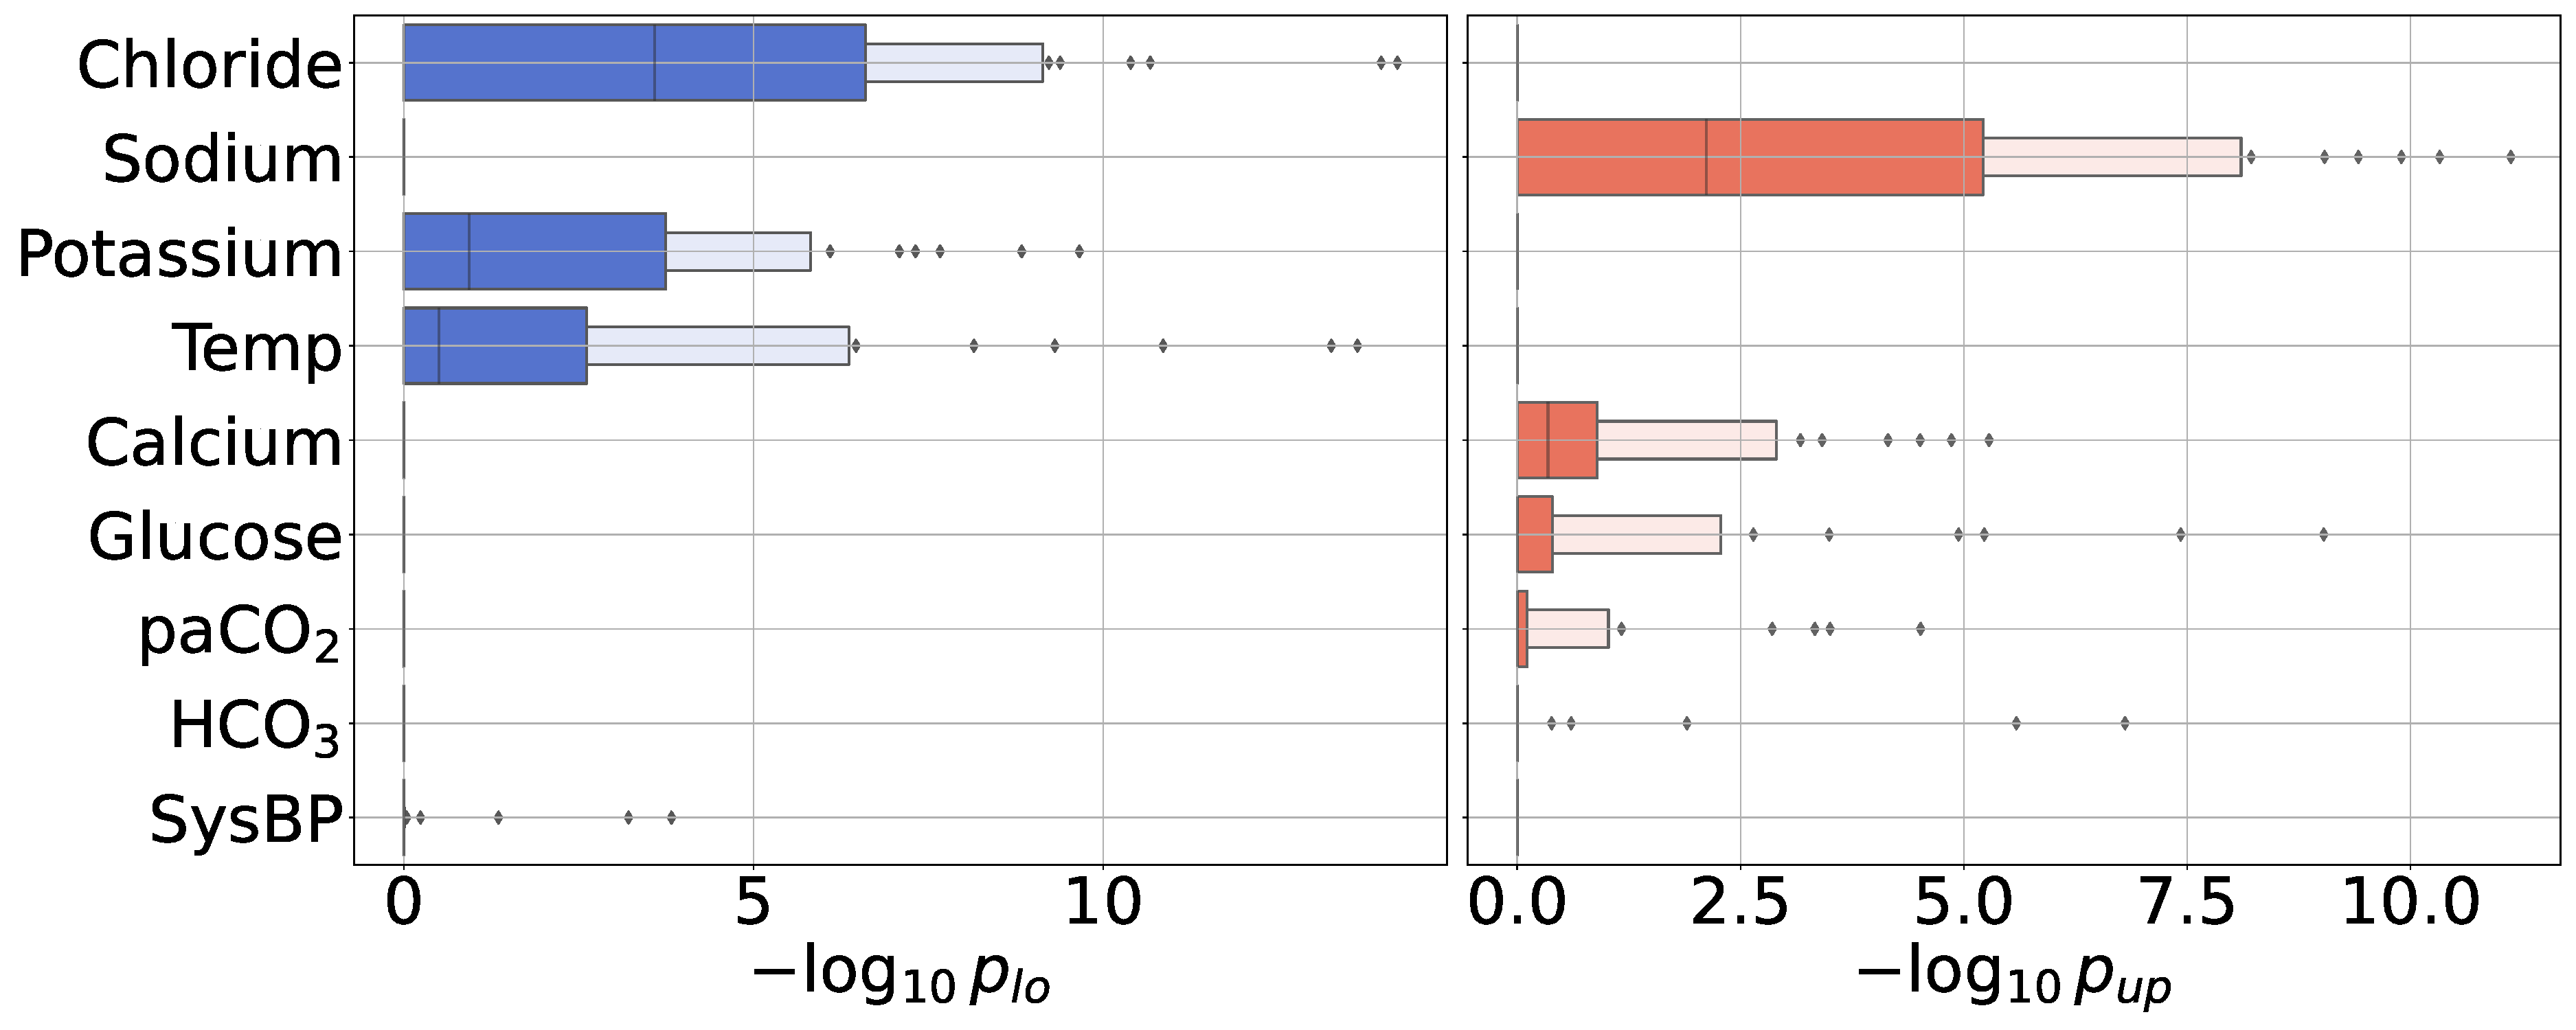
\includegraphics[height=4.5cm]{figures/causal/latest_experimental_results/p_values_nogray.pdf}
    \caption{Distributions of $-\log_{10}{p_\textup{lo}}$ and $-\log_{10}{p_\textup{up}}$ across hypotheses, grouped by physiological quantity. Higher values indicate greater evidence in favour of rejection.}
    \label{fig:p_values}
\end{figure}



\subsection{Pitfalls of naive assessment}

A naive approach to twin assessment involves simply comparing the output of the twin with the observational data directly, without accounting for causal considerations.
We now show that, unlike our methodology, the results produced in this way can be potentially misleading.
% assessing the twin in this straightforward way can be misleading.
In Figure \ref{fig:longitudinal_plots}, for two different choices of $(\ax_{1:4}, \B_{1:4})$, we plot estimates of $\Qt_\tx$ and $\Q^{\textup{obs}}_\tx$ for $\tx \in \{1, \ldots, 4\}$, where
% \begin{small}
\begin{align*}
    \Qt_\tx &\coloneqq \E[\Yt(\ax_{1:\tx})\mid \X_0 \in \B_0, \Xt_{1:\tx}(\X_0, \ax_{1:\tx}) \in \B_{1:\tx}] \\
    \Q^{\textup{obs}}_\tx &\coloneqq \E[\Y(\A_{1:\tx})\mid \X_{0:\tx}(\A_{1:\tx})\in \B_{0:\tx}, \A_{1:\tx}=\ax_{1:\tx}].
\end{align*}
\begin{figure}%[h!]
    \centering
    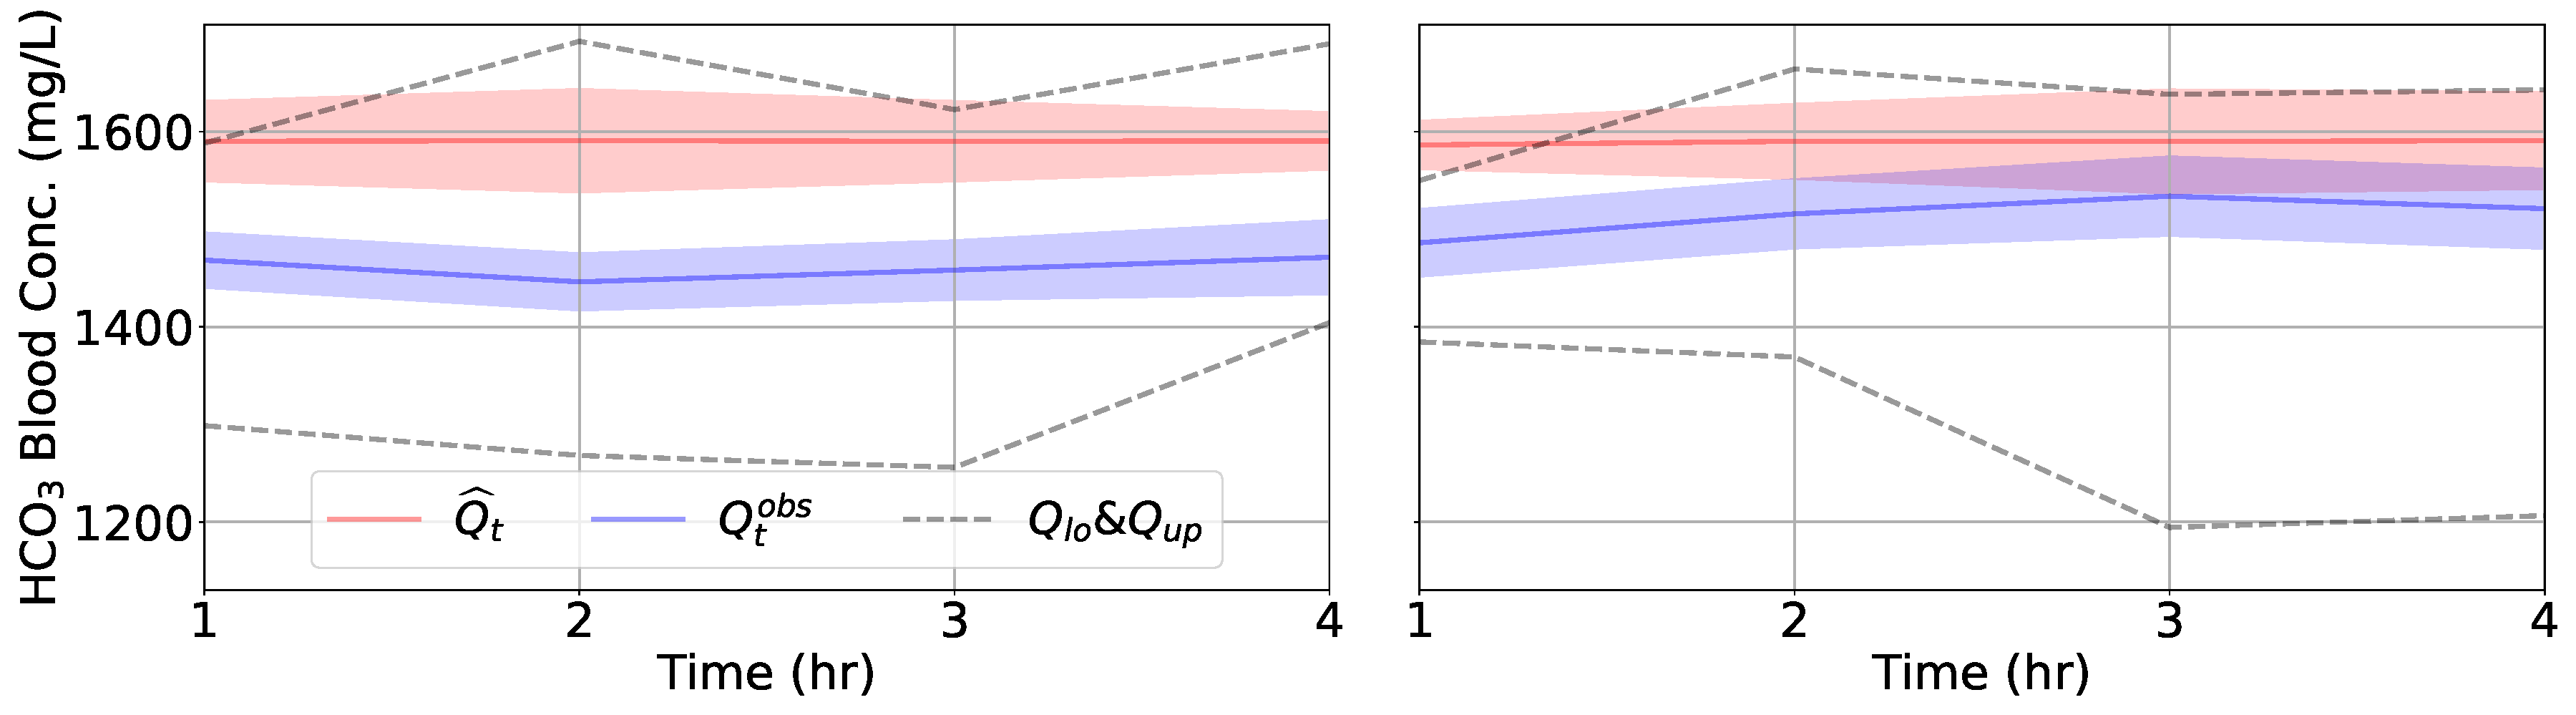
\includegraphics[height=4cm]{figures/causal/longitudinal_plots/HCO3_hyp_38v37_longitudinal_nogray.pdf}
    \caption{Estimates and 95\% confidence intervals for $\Qt_\tx$ and $\Q^{\textup{obs}}_\tx$ at each $1\leq \tx \leq 4$ for two choices of $(\B_{0:4}, \ax_{1:4})$, where $\Yt(\ax_{1:\tx})$ and $\Y(\ax_{1:\tx})$ correspond to HCO$_3$ concentration.
    The dashed lines indicate lower and upper 95\% confidence intervals for $\Qlo, \Qup$ respectively.  }
    \label{fig:longitudinal_plots}
\end{figure}
% \end{small}
% \begin{eqnarray*}
%     \Qt_\tx &\coloneqq& \E[\Yt(\ax_{1:\tx})\mid \X_0 \in \B_0, \Xt_{1:\tx}(\X_0, \ax_{1:\tx}) \in \B_{1:\tx}]\\
%     \Q^{\textup{obs}}_\tx &\coloneqq& \E[\Y(\A_{1:\tx})\mid \X_{0:\tx}(\A_{1:\tx})\in \B_{0:\tx}, \A_{1:\tx}=\ax_{1:\tx}].
% \end{eqnarray*}
Here $\Qt_\tx$ is just $\Qt$ as defined above with its dependence on $\tx$ made explicit.
Each plot also shows one-sided 95\% confidence intervals on $\Qlo$ and $\Qup$ at each $\tx \in \{1, \ldots, 4\}$ obtained from Hoeffding's inequality. 
Directly comparing the estimates of $\Qt_\tx$ and $\Q^{\textup{obs}}_\tx$ would suggest that the twin is comparatively more accurate for the right-hand plot, as these estimates are closer to one another in that case.
However, the output of the twin in the right-hand plot is falsified at $\tx = 1$, as can be seen from the fact that confidence interval for $\Qt_1$ lies entirely above the one-sided confidence interval for $\Qup$ at that timestep.
On the other hand, the output of the twin in the left-hand plot is not falsified at any of the timesteps shown, so that the twin may in fact be accurate for these $(\ax_{1:4}, \B_{1:4})$, contrary to what a naive assessment strategy would suggest.
Our methodology provides a principled means for twin assessment that avoids drawing potentially misleading inferences like this.


A similar phenomenon appears in Figure \ref{fig:histograms}, which for two choices of $\B_{0:\tx}$ and $\ax_{1:\tx}$ shows histograms of raw glucose values obtained from the observational data conditional on $\A_{1:\tx}=\ax_{1:\tx}$ and $\X_{0:\tx}(\A_{1:\tx})\in \B_{0:\tx}$, and from the twin conditional on $\Xt_{0:\tx}(\ax_{1:\tx})\in \B_{0:\tx}$.
% (Note that these raw values differ slightly from $\Y(\A_{1:\tx})$ and $\Yt(\ax_{1:\tx})$ since they are not clipped to lie between $\ylo$ and $\yup$.)
% $\Yt(\ax_{1:\tx})$ conditional on $\Xt_{0:\tx}(\ax_{1:\tx})\in \B_{0:\tx}$, and of $\Y(\A_{1:\tx})$ conditional on $\A_{1:\tx}=\ax_{1:\tx}$ and $\X_{0:\tx}(\A_{1:\tx})\in \B_{0:\tx}$.
Below each histogram we also show 95\% confidence intervals for $\Qup$ and $\Qt$ obtained from Hoeffding's inequality.
While Figures \ref{fig:glucosea} and \ref{fig:glucoseb} appear visually very similar, the inferences produced by our testing procedure are different: the hypothesis corresponding to the right-hand plot is rejected, since there is no overlap between the confidence intervals underneath, while the hypothesis corresponding to the left-hand plot is not.
This was not an isolated case and several other examples of this phenomenon are shown in Figure \ref{fig:histograms-supplement} in the \AppendixName. 
This demonstrates that the inferences obtained from our procedure do not depend only on the distribution of observed outcomes (which is essentially the same for both cases).
Instead, as discussed in Section \ref{sec:causal-bounds-statement}, these also account for the worst-case effects of unmeasured confounding that may exist in the observational data.

% range of possible outcomes that might have been observed in the data 
% worst-case outcomes that may possibly occur in the presence of unmeasured confounding.

% these also depend on the value of $\Prob(\A_{1:\tx} = \ax_{1:\tx} \mid \X_{0:\tx}(\A_{1:\N}))$

% also account for the fact that the data might be confounded, and therefore may take on the worst-case values $\ylo$ and $\yup$

% possibility of confounding in the data.

% observational distribution of the data .
% not simply rely on direct comparison of observed and simulated trajectories, but 

% A similar phenomenon appears in Figure \ref{fig:histograms}, which, for two choices of $\B_{0:\tx}$ and $\ax_{1:\tx}$, shows histograms of $\Yt(\ax_{1:\tx})$ conditional on $\Xt_{0:\tx}(\ax_{1:\tx})\in \B_{0:\tx}$, and of $\Y(\A_{1:\tx})$ conditional on $\A_{1:\tx}=\ax_{1:\tx}$ and $\X_{0:\tx}(\A_{1:\tx})\in \B_{0:\tx}$.
% We also include 95\% confidence intervals for $\Qlo$ and $\Qt$ obtained from Hoeffding's inequality.
% While Figures \ref{fig:glucosea} and \ref{fig:glucoseb} appear visually very similar, the inferences produced by our testing procedure are different: the hypothesis corresponding to the right-hand plot is rejected, since there is no overlap between the confidence intervals underneath, while the hypothesis corresponding to the left-hand plot is not.
% We give a similar example in Section \ref{sec:experiments-supplement} of the \AppendixName.
% This demonstrates that our methodology does not simply rely on direct comparison of observed and simulated outcomes, but also accounts for the possibility of arbitrary confounding in the data.





\begin{figure}%[h!]
    \centering
    \begin{subfigure}[b]{0.5\textwidth}
    \centering
    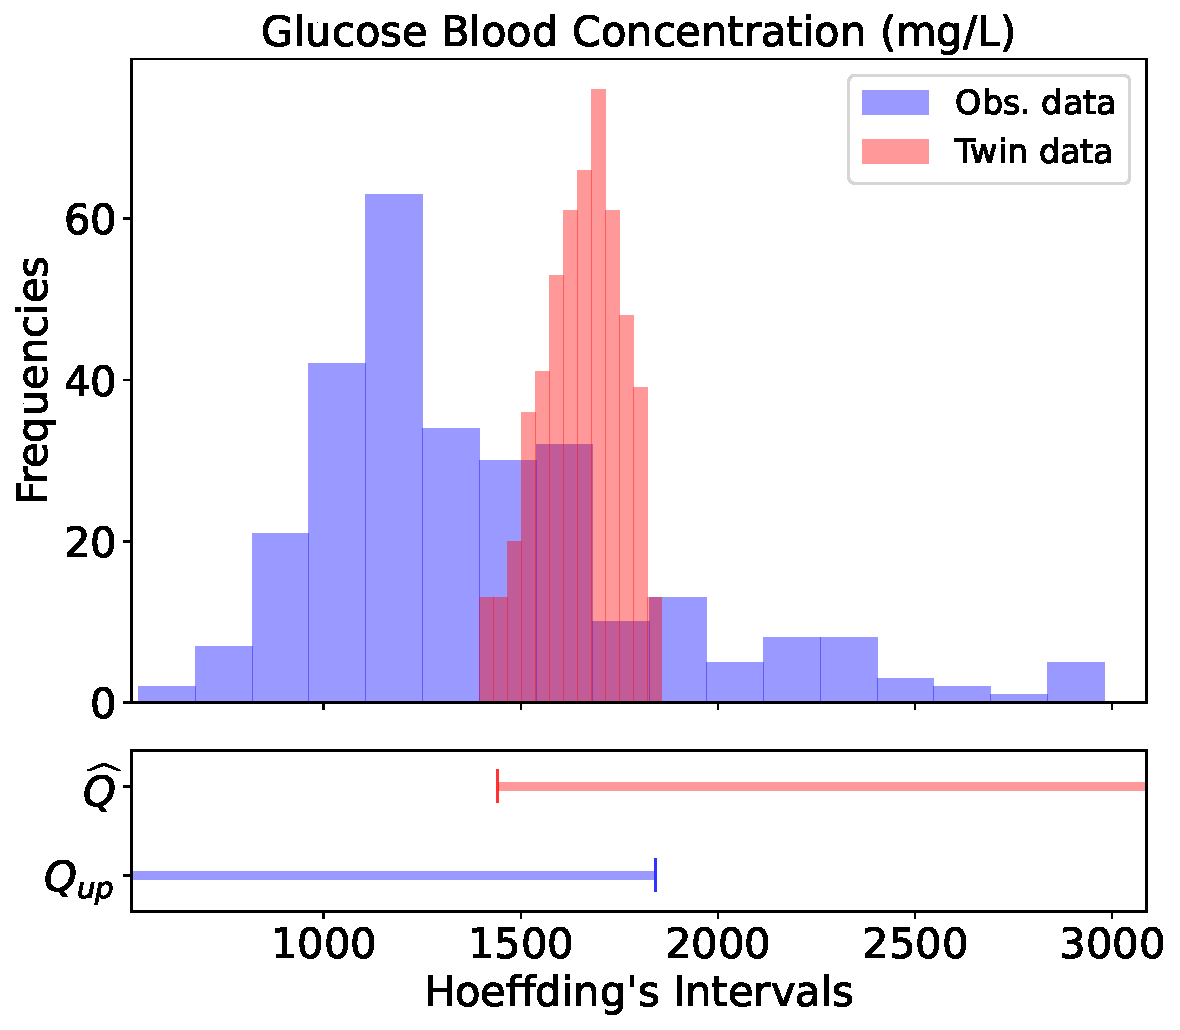
\includegraphics[height=5cm]{figures/causal/latest_experimental_results/truncated_hists/Glucose_hyp_1_with_hoeff_onesided_loFalse_p0.2_nogray.pdf}
    \subcaption{Not rejected}
    \label{fig:glucosea}
    \end{subfigure}%
    \begin{subfigure}[b]{0.5\textwidth}
    \centering
    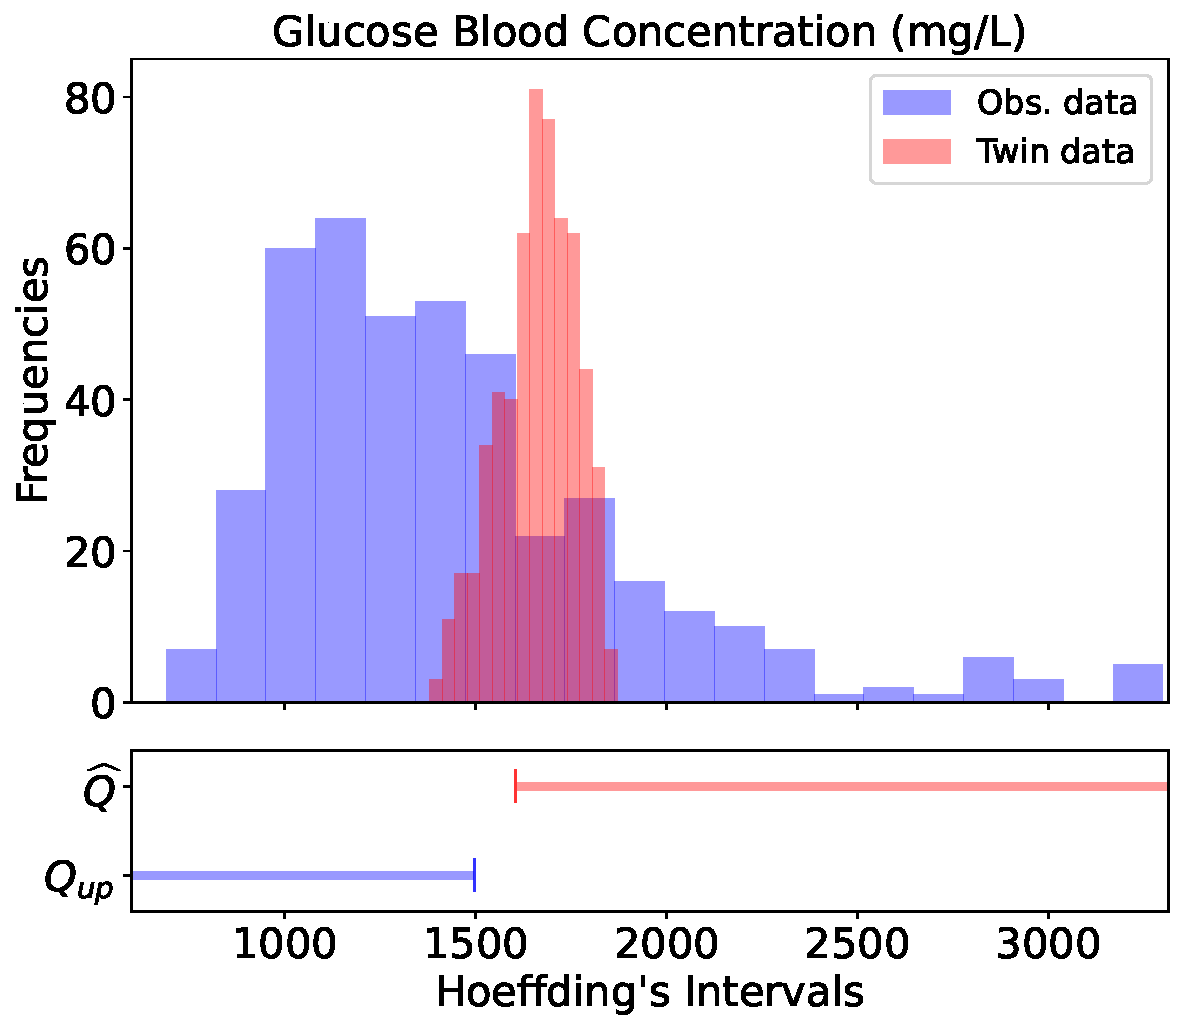
\includegraphics[height=5cm]{figures/causal/latest_experimental_results/truncated_hists/Glucose_hyp_5_with_hoeff_onesided_loFalse_p0.2_nogray.pdf}
    \subcaption{Rejected}
    \label{fig:glucoseb}
    \end{subfigure}
    %     \begin{subfigure}[b]{0.25\textwidth}
    % \includegraphics[height=3.5cm]{figures/causal/Glucose_hyp_8_with_hoeff_onesided_loFalse_p0.2_untruncated.pdf}
    % \subcaption{Not rejected}
    % \label{fig:glucosec}
    % \end{subfigure}%
    % \begin{subfigure}[b]{0.25\textwidth}
    % \includegraphics[height=3.5cm]{figures/causal/Glucose_hyp_6_with_hoeff_onesided_loFalse_p0.2_untruncated.pdf}
    % \subcaption{Rejected}
    % \label{fig:glucosed}
    % \end{subfigure}     
    \caption{Raw glucose values from the observational data and twin for two choices of $(\B_{0:\tx}, \ax_{1:\tx})$, with confidence intervals for $\Qt$ and $\Qup$ shown below. The horizontal axes are truncated to the .025 and .975 quantiles of the observational data for clarity. Untruncated plots are shown in Figure \ref{fig:histograms-supplement} of the \AppendixName.}
    % to make visually clearer whether or not the confidence intervals overlap. \rob{Refer to untruncated Figure in supplement}}
    % $\Yt(\ax_{1:\tx})$ conditional on $\Xt_{0:\tx}(\ax_{1:\tx})\in \B_{0:\tx}$, and of $\Y(\A_{1:\tx})$ conditional on $\A_{1:\tx}=\ax_{1:\tx}$ and $\X_{0:\tx}(\A_{1:\tx})\in \B_{0:\tx}$ for two hypotheses with Glucose as outcome. Below each figure we also provide Hoeffding 95\% confidence intervals for the corresponding hypotheses. \faaiz{For illustrative purposes the histograms of $\Y(\A_{1:\tx})$ have been truncated between .025 and .975 quantiles.}}
        % \caption{Histograms of $\Yt(\ax_{1:\tx})$ conditional on $\Xt_{0:\tx}(\ax_{1:\tx})\in \B_{0:\tx}$, and of $\Y(\A_{1:\tx})$ conditional on $\A_{1:\tx}=\ax_{1:\tx}$ and $\X_{0:\tx}(\A_{1:\tx})\in \B_{0:\tx}$ for two hypotheses with Glucose as outcome. Below each figure we also provide Hoeffding 95\% confidence intervals for the corresponding hypotheses. \faaiz{For illustrative purposes the histograms of $\Y(\A_{1:\tx})$ have been truncated between .025 and .975 quantiles.}}
    \label{fig:histograms}
\end{figure}


\section{Discussion}

We have advocated for a causal approach to digital twin assessment, and have presented a statistical procedure for doing so that obtains rigorous theoretical guarantees under minimal assumptions.
We now highlight the key limitations of our approach.
Importantly, our methodology implicitly assumes that there is no distribution shift between testing and deployment time.
% the interventional distribution of the real-world process does not differ between when our dataset was obtained and when the twin is deployed to production. % Most significantly, our methodology implicitly assumes that the distribution of data used to assess the twin is the same as the distribution of data that will be observed when the twin is deployed to production.
% data used to assess the twin is the same as the distribution of data that will be observed when the twin is deployed to production.
If the conditional distribution of $\X_{1:\T}(\ax_{1:\T})$ given $\X_0$ changes at deployment time, then so too does the set of twins that are interventionally correct, and if this change is significant enough, our assessment procedure may yield misleading results.
% This may occur in cases where $\X_0$ encodes previous actions that were taken before $\tx = 0$, which is useful in certain decision-support cases (see Section \ref{sec:online-prediction} of the \AppendixName).
% \faaiz{vague}
% In such cases, distribution shift can arise if the policy used to determine these historical actions changes at deployment time.
% This may occur for example if at deployment time the values of $\X_0$ used to initialise the twin trajectories encode previous actions chosen according to a considerably different policy than the behavioural agent's policy in observational data. We outline certain decision-support settings in which this may occur in Section \ref{sec:online-correctness-alternative-notion-supp} of the \AppendixName.
% chosen by some behavioural agent whose policy differs from the one used to collect observational data for our assessment procedure.
% This may occur for example with twins whose $\X_0$ encodes previous confounded actions chosen by some behavioural agent (which may occur in certain decision-support settings as described in Section \ref{sec:online-correctness-alternative-notion-supp} of the \AppendixName) if the policy of that agent changes considerably before deployment.
Distribution shift in this sense is a separate issue to unobserved confounding, and arises in a wide variety of statistical problems beyond ours.

Additionally, the procedure we used in our case study to choose the hypothesis parameters $\B_{0:\tx}$ was ad hoc.
For scalability, it would likely be necessary to obtain $\B_{0:\tx}$ via a more automated procedure.
It may also be desirable to choose $\B_{0:\tx}$ dynamically in light of previous hypotheses tested, zooming in to regions containing possible failure modes to obtain increasingly granular information about the twin.
We see opportunities here for using machine learning techniques, but leave this to future work.

% We see opportunities for doing so using machine learning techniques, which may lead to more informative hypotheses, or more powerful tests.


% Additionally, our procedure for choosing $\B_{0:\T}$ is somewhat crude.
% We expect more informative hypotheses could be obtained by 


% Additionally, as a statistical method, our approach to twin assessment can only yield statements about how well the twin performs on average across some (potentially hypothetical) population of interest.
% In particular, our methodology cannot determine how well or how poorly the twin  will predict the future of any specific unit in the population.
% Mathematically, this is expressed in the way we consider the distribution of outputs of the twin $\Xt_{1:\T}(\X_0, \ax_{1:\T})$, rather than its almost sure behaviour.
% That said, if our assessment indicates that the twin does poorly on average across the population, then it must necessarily do so for a large proportion of its units, which would give reason for mistrusting the outputs of the twin on any specific individual.

Various other extensions and improvements appear possible.
For example, 
% it is possible to replace our one-sided confidence intervals for $\Qlo$, $\Qup$, and $\Qt$ with two-sided ones, and thereby to obtain a procedure that may yield more precise information about the twin than we obtain by rejecting one of $\Hlo$ or $\Hup$.
% We outline this at a high level in Section \ref{sec:two-sided-intervals-supplement} of the \AppendixName.
one can leverage ideas from the literature on partial identification \citep{manski2003partial} to obtain greater statistical efficiency, for example by building on the line of work initiated by \cite{imbens2004confidence} for obtaining more informative confidence intervals.
% We also perceive opportunities for leveraging ideas from the literature on partial identification \cite{manski2003partial} to obtain a more efficient statistical procedure, for example by building on the line of work initiated by \cite{imbens2004confidence} for obtaining more informative confidence intervals in this context.
% One concrete possibility would be to consider techniques based on confidence intervals that cover directly the non-identified parameter $\Q$ in the manner proposed by \cite{imbens2004confidence}, which are more informative than intervals that cover the entire identified region $[\Qlo, \Qup]$ as we use.
Beyond this, it may sometimes be useful to consider additional assumptions that lead to less conservative assessment results.
For example, various methods for \emph{sensitivity analysis} have been proposed that model the \emph{degree} to which the actions of the behavioural agent are confounded \citep{rosenbaum2002observational,tan2006distributional,yadlowsky2022bounds}.
This can yield tighter bounds on $\Q$ than are implied by Theorem \ref{thm:causal-bounds}, albeit at the expense of less robustness if these assumptions are violated.


% Various extensions and improvements to our approach also appear possible.
% For example, it is possible to replace our one-sided confidence intervals for $\Qlo$, $\Qup$, and $\Qt$ with two-sided ones, and thereby to obtain a procedure that may yield more precise information about the twin than we obtain by rejecting one of $\Hlo$ or $\Hup$.
% We describe this at a high level in Section \ref{sec:two-sided-intervals-supplement} of the \AppendixName.
% Additionally, our procedure for choosing $\B_{0:\T}$ is somewhat crude.
% We expect more informative hypotheses could be obtained by choosing $\B_{0:\T}$ dynamically in light of previous hypotheses tested, zooming in to regions containing possible failure modes in order to obtain even more granular information about the twin.
% We also perceive various opportunities for leveraging ideas from the literature on partial identification \cite{manski2003partial} to obtain more efficient statistical procedures, for example by building on the line of work initiated by \cite{imbens2004confidence} for obtaining more informative confidence intervals in this context.
% % One concrete possibility would be to consider techniques based on confidence intervals that cover directly the non-identified parameter $\Q$ in the manner proposed by \cite{imbens2004confidence}, which are more informative than intervals that cover the entire identified region $[\Qlo, \Qup]$ as we use.
% Beyond this, it may be useful in certain contexts to add more assumptions to the model so as to obtain more informative assessment results.
% One approach to doing so is based on modelling the \emph{degree} to which the actions of the behavioural agent are confounded, which can lead to tighter bounds on $\Q$ than are implied by Theorem \ref{thm:causal-bounds} \cite{rosenbaum2002observational,tan2006distributional, namkoong2020offpolicy,kallus2018confounding}, albeit at the expense of less robustness if these assumptions in fact turn out to be violated.

% To do